\chapter{Anhang}

\section{Architekturen}

\begin{figure}
	\centering
	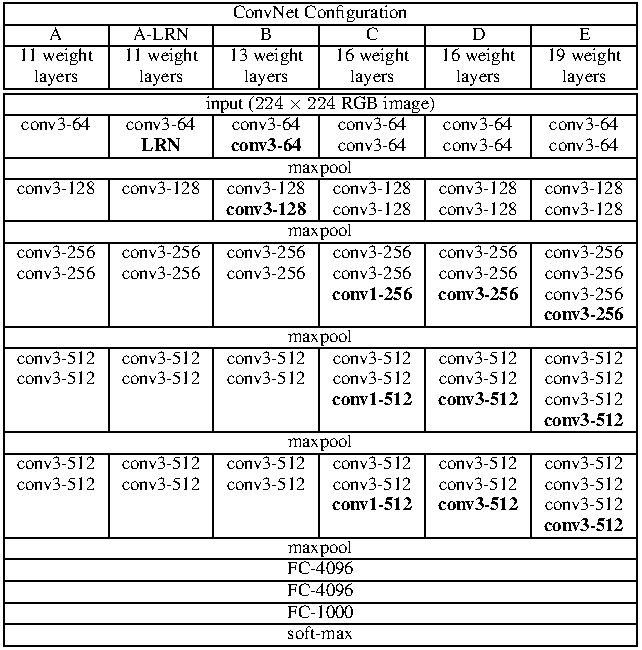
\includegraphics[width=0.8\textwidth]{Bilder/vgg16-architecture.pdf} 
	\caption{Die ursprünglichen VGG-Architekturen. Spalte D zeigt VGG16 wie in \autoref{sec:pretrained-backbones:vgg16} beschrieben. Abb. aus \cite{Simonyan.04092014}.}
	\label{fig:vgg16-architecture}
\end{figure} 

\begin{figure}
	\centering
	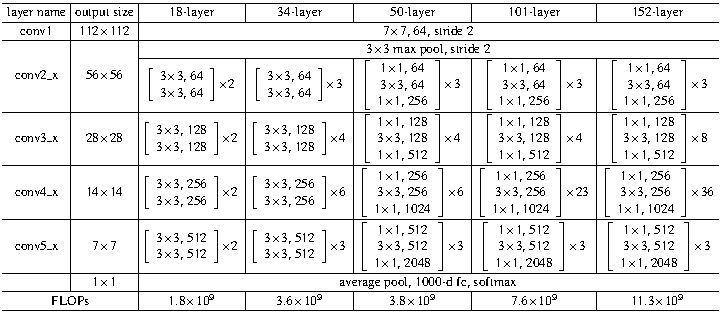
\includegraphics[width=0.8\textwidth]{Bilder/resnet34-architecture.pdf} 
	\caption{Die ursprünglichen ResNet-Architekturen. Zwischen jeweils zwei Convolutional-Layer befindet sich eine Skip-Connection \cite{He.10122015}.}
	\label{fig:resnet34-architecture}
\end{figure} 

\begin{figure}
	\centering
	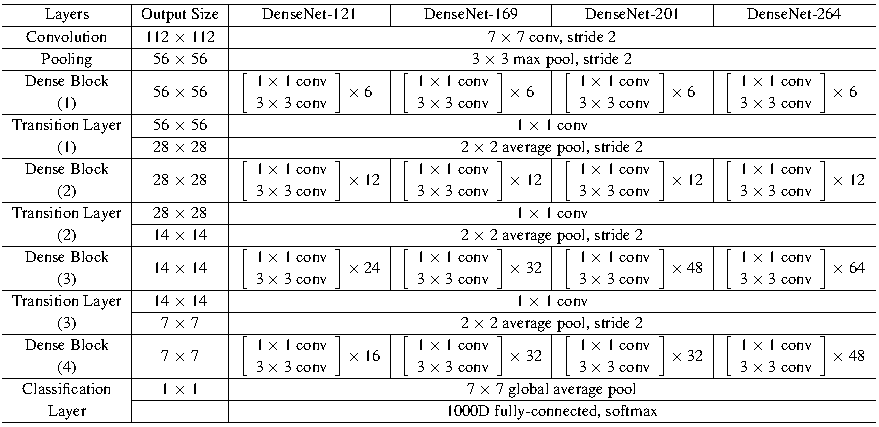
\includegraphics[width=0.8\textwidth]{Bilder/densenet121-architecture.pdf} 
	\caption{Die ursprünglichen DenseNet-Architekturen \cite{Huang.25082016}.}
	\label{fig:densenet121-architecture}
\end{figure} 

\pagebreak

\section{Quelltext-Implementation}

\lstinputlisting[
	label=code:quality,    % Label; genutzt für Referenzen auf dieses Code-Beispiel
	caption=Implementation des Quality-Maßes in Python zur Verwendung im Training und Testen von Keras-Modellen.,
	captionpos=b,               % Position, an der die Caption angezeigt wird t(op) oder b(ottom)
	style=EigenerPythonStyle,   % Eigener Style der vor dem Dokument festgelegt wurde
	firstline=1,                % Zeilennummer im Dokument welche als erste angezeigt wird
	lastline=50                 % Letzte Zeile welche ins LaTeX Dokument übernommen wird
]{Quellcode/quality.py}

\pagebreak 

\section{Beispiel-Predictions Combined} \label{sec:pred-combined}


\begin{figure}
	\centering
	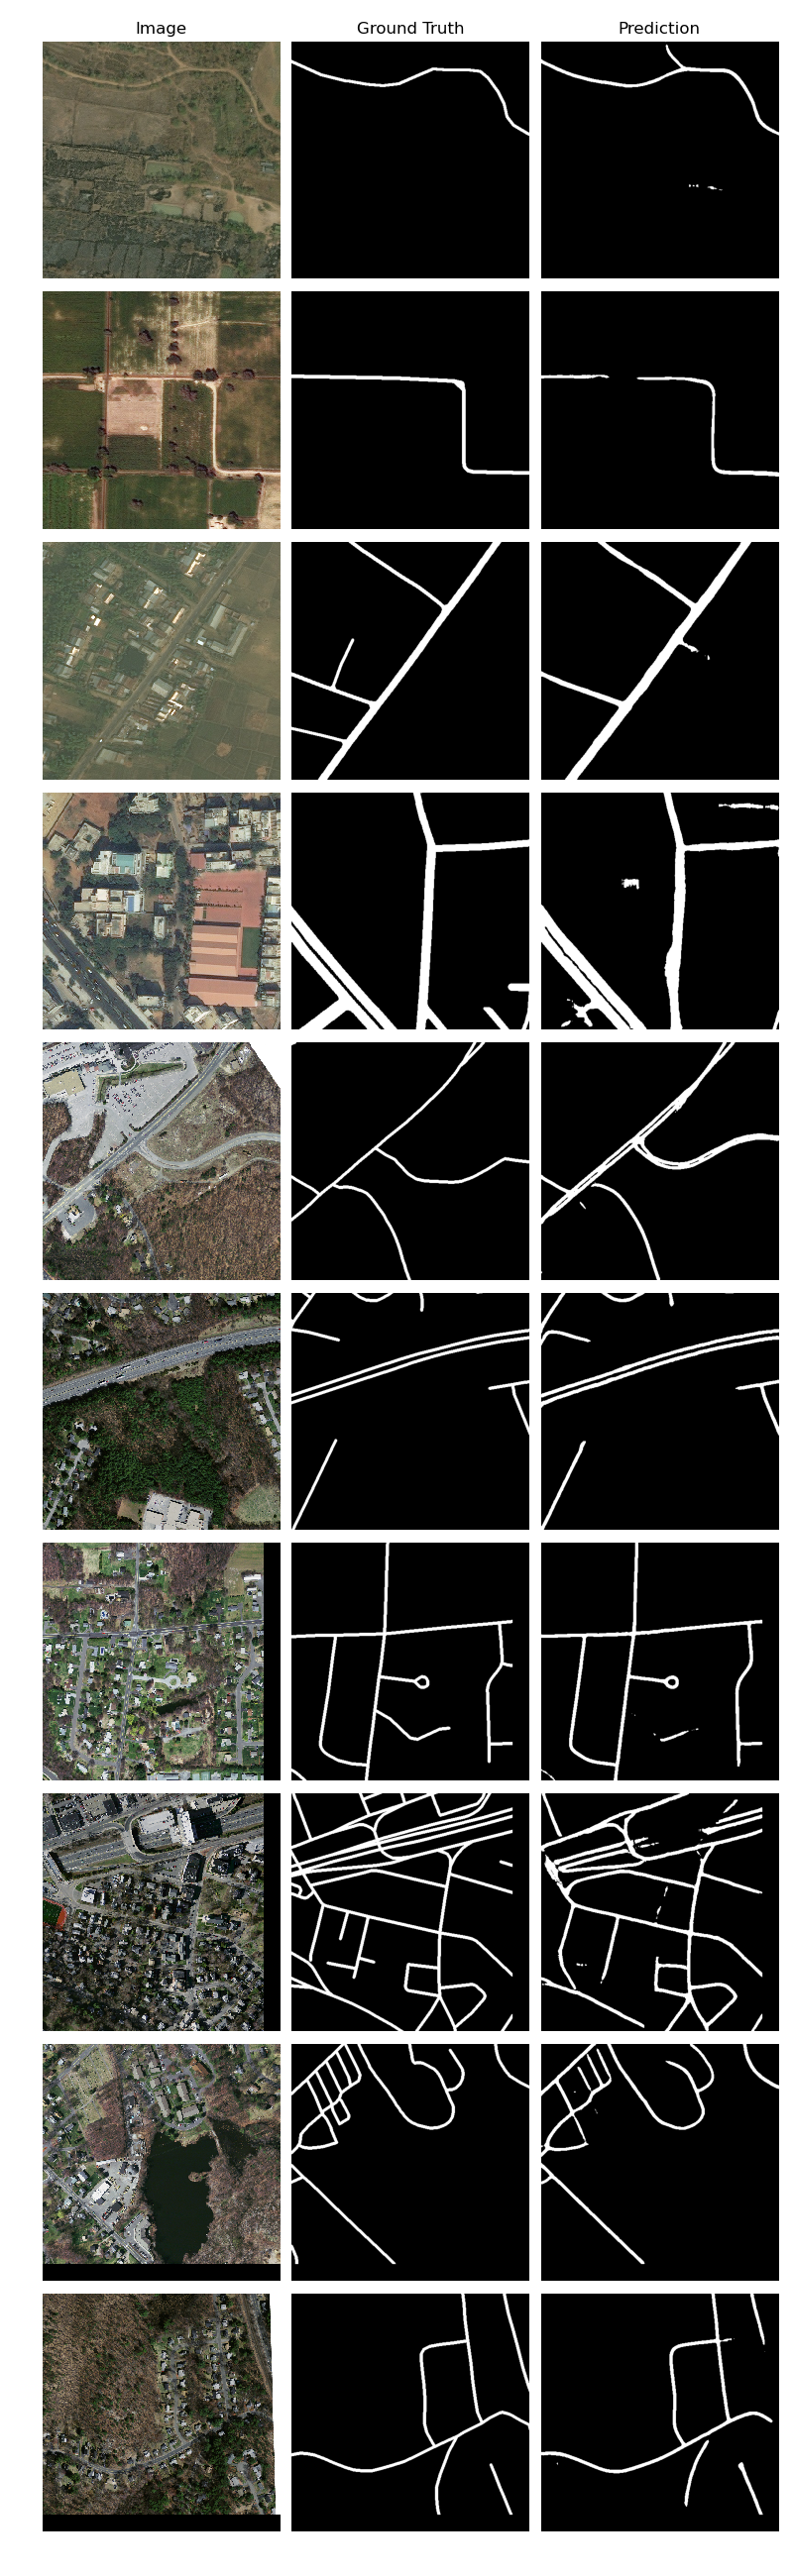
\includegraphics[width=.41\textwidth]{Bilder/Samples-Combined/bunet15.png}
	\caption{Beispiel-Predictions des $BUNet15$ auf dem Combined-Datensatz.}
	\label{fig:combined-samples-bunet15}
\end{figure}

\begin{figure}
	\centering
	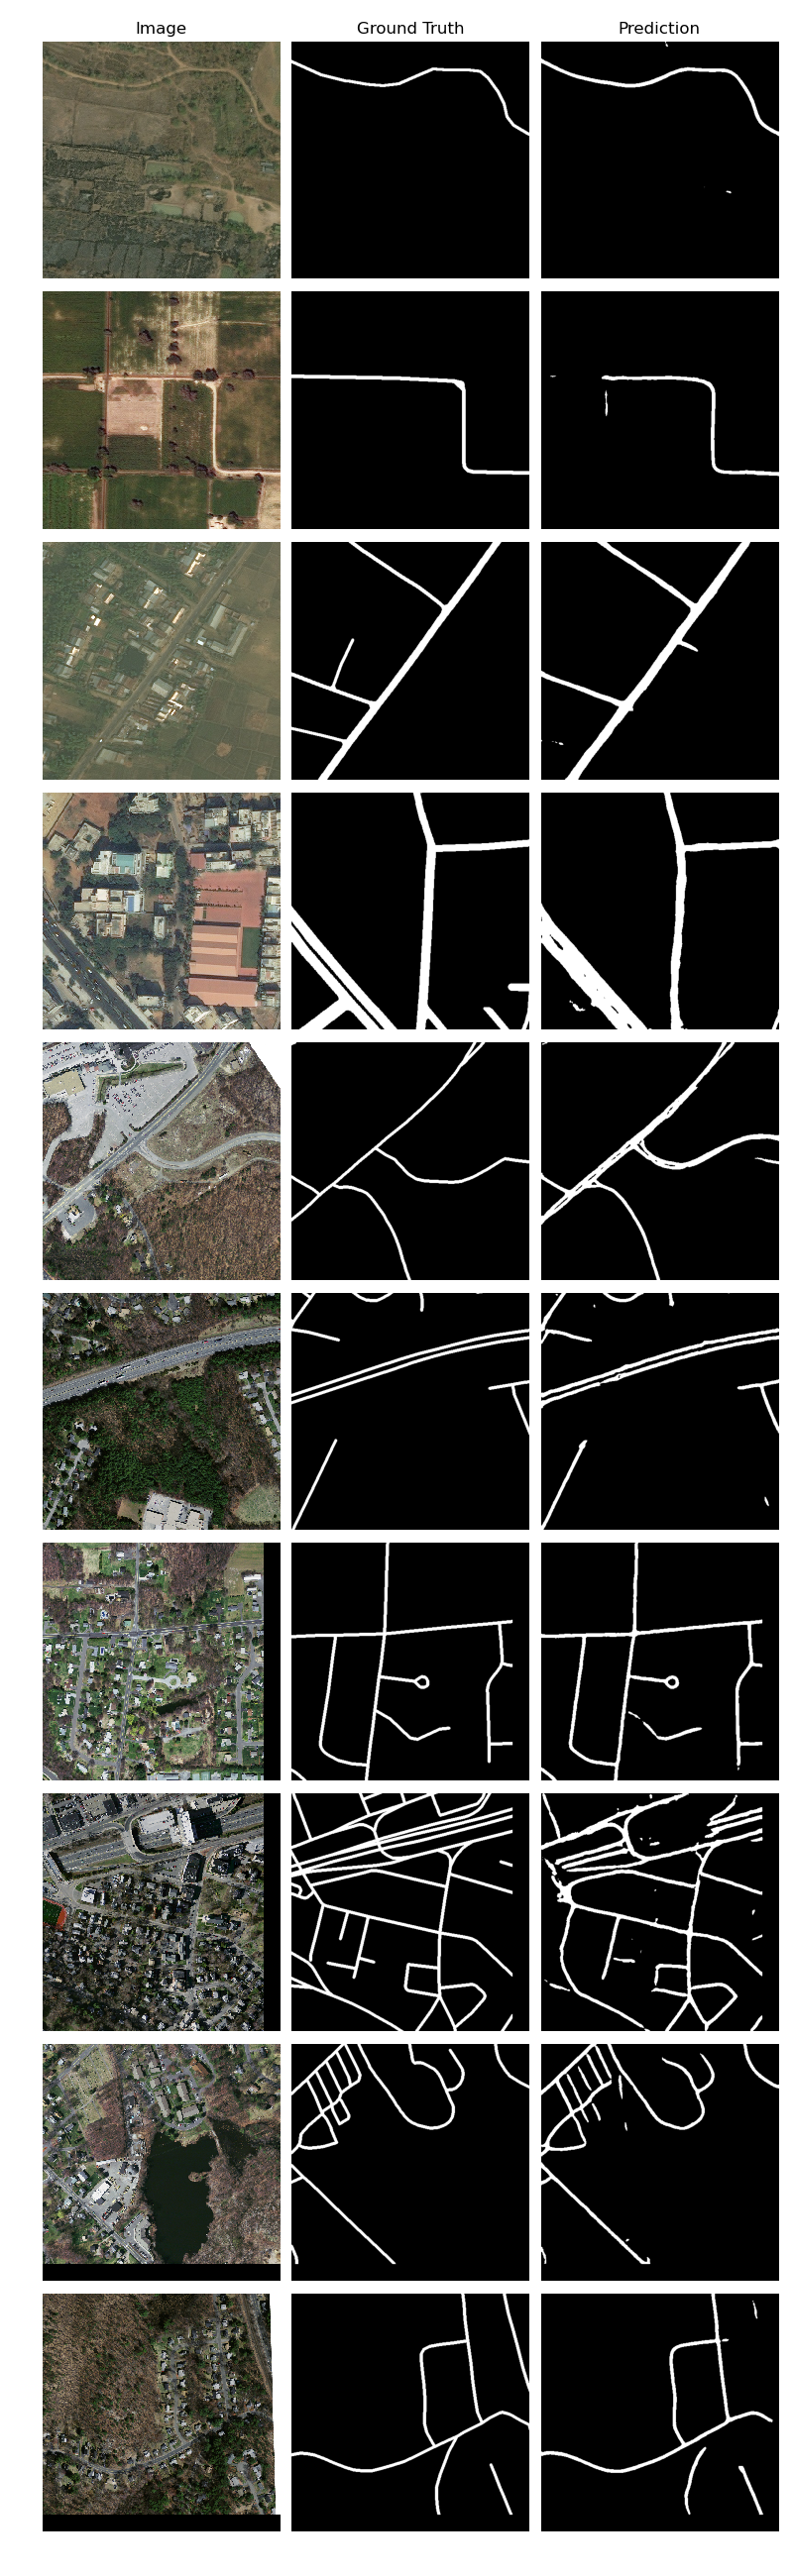
\includegraphics[width=.41\textwidth]{Bilder/Samples-Combined/dbunet.png}
	\caption{Beispiel-Predictions des $DBUNet$ auf dem Combined-Datensatz.}
	\label{fig:combined-samples-dbunet}
\end{figure}

\begin{figure}
	\centering
	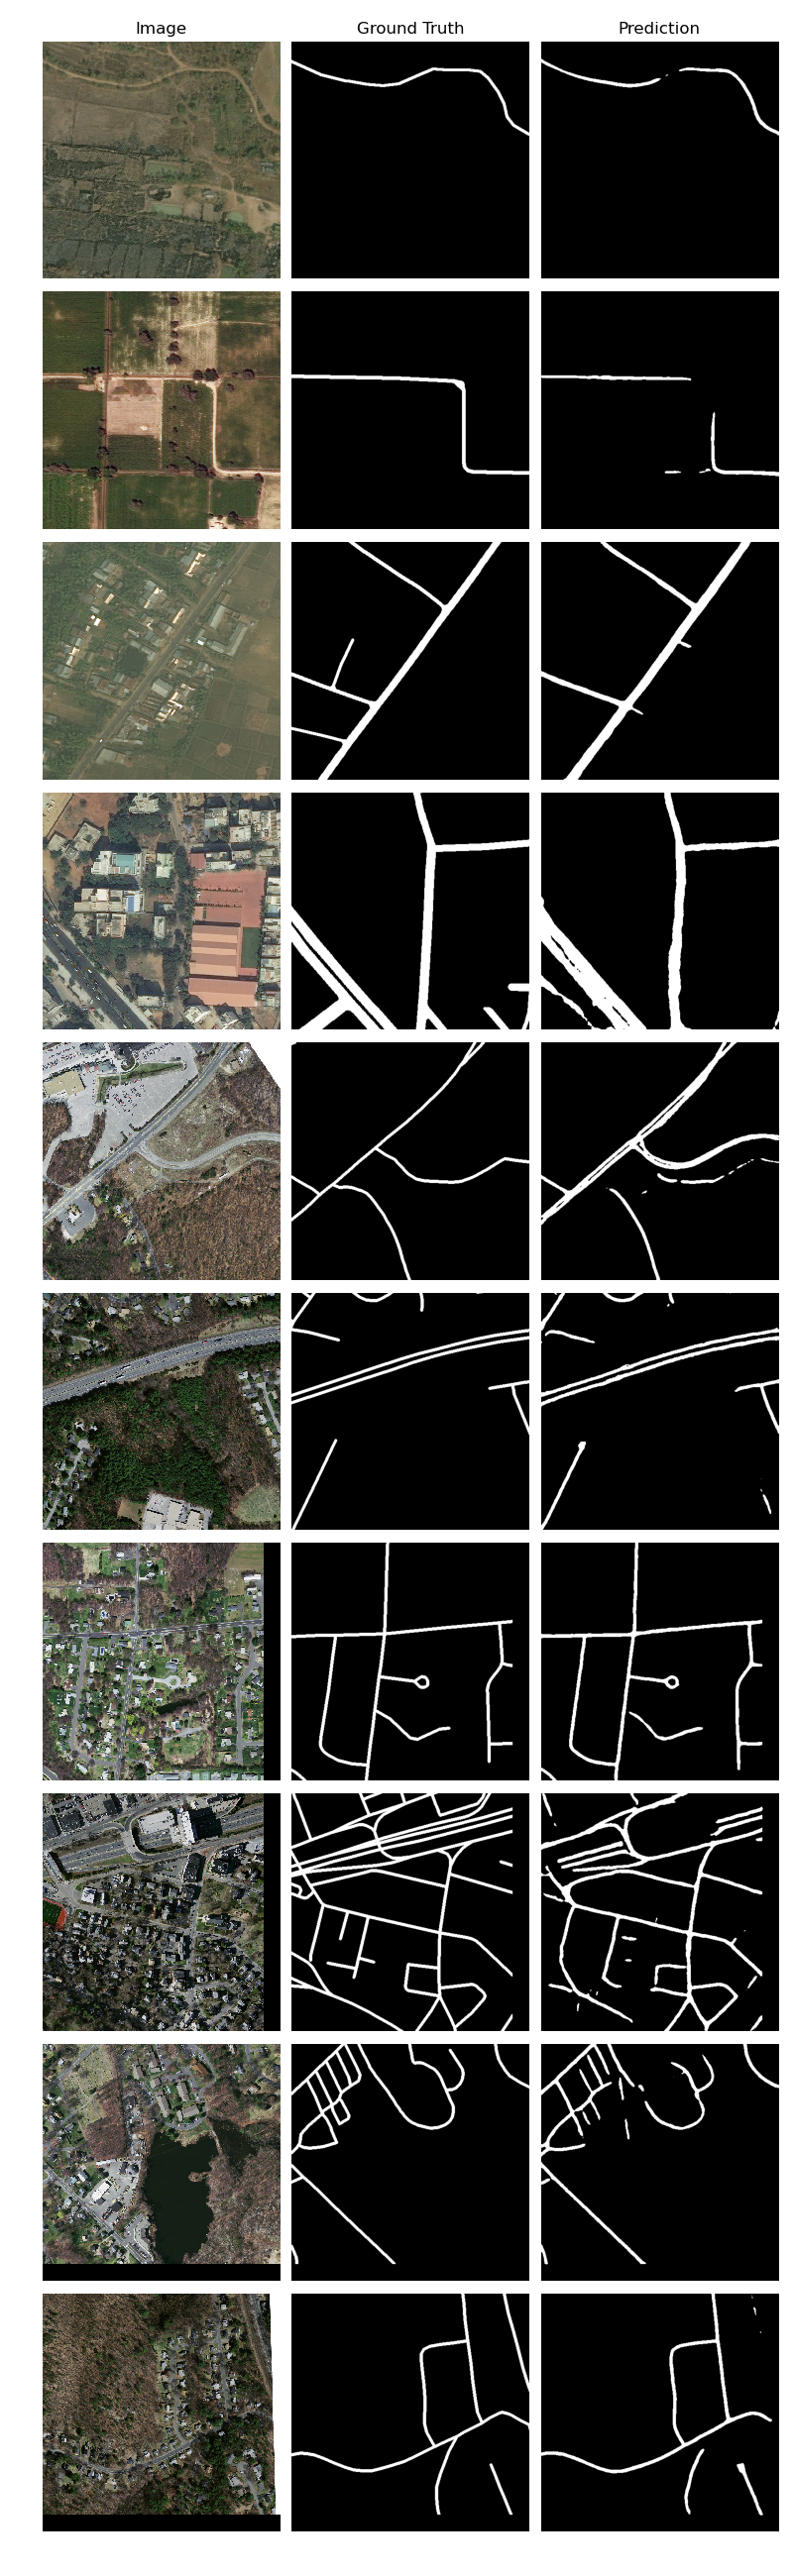
\includegraphics[width=.41\textwidth]{Bilder/Samples-Combined/rbunet.png}
	\caption{Beispiel-Predictions des $RBUNet$ auf dem Combined-Datensatz.}
	\label{fig:combined-samples-rbunet}
\end{figure}



\pagebreak 



\section{Beispiel-Predictions BikeSat} \label{sec:pred-bikesat}

\begin{figure}
	\centering
	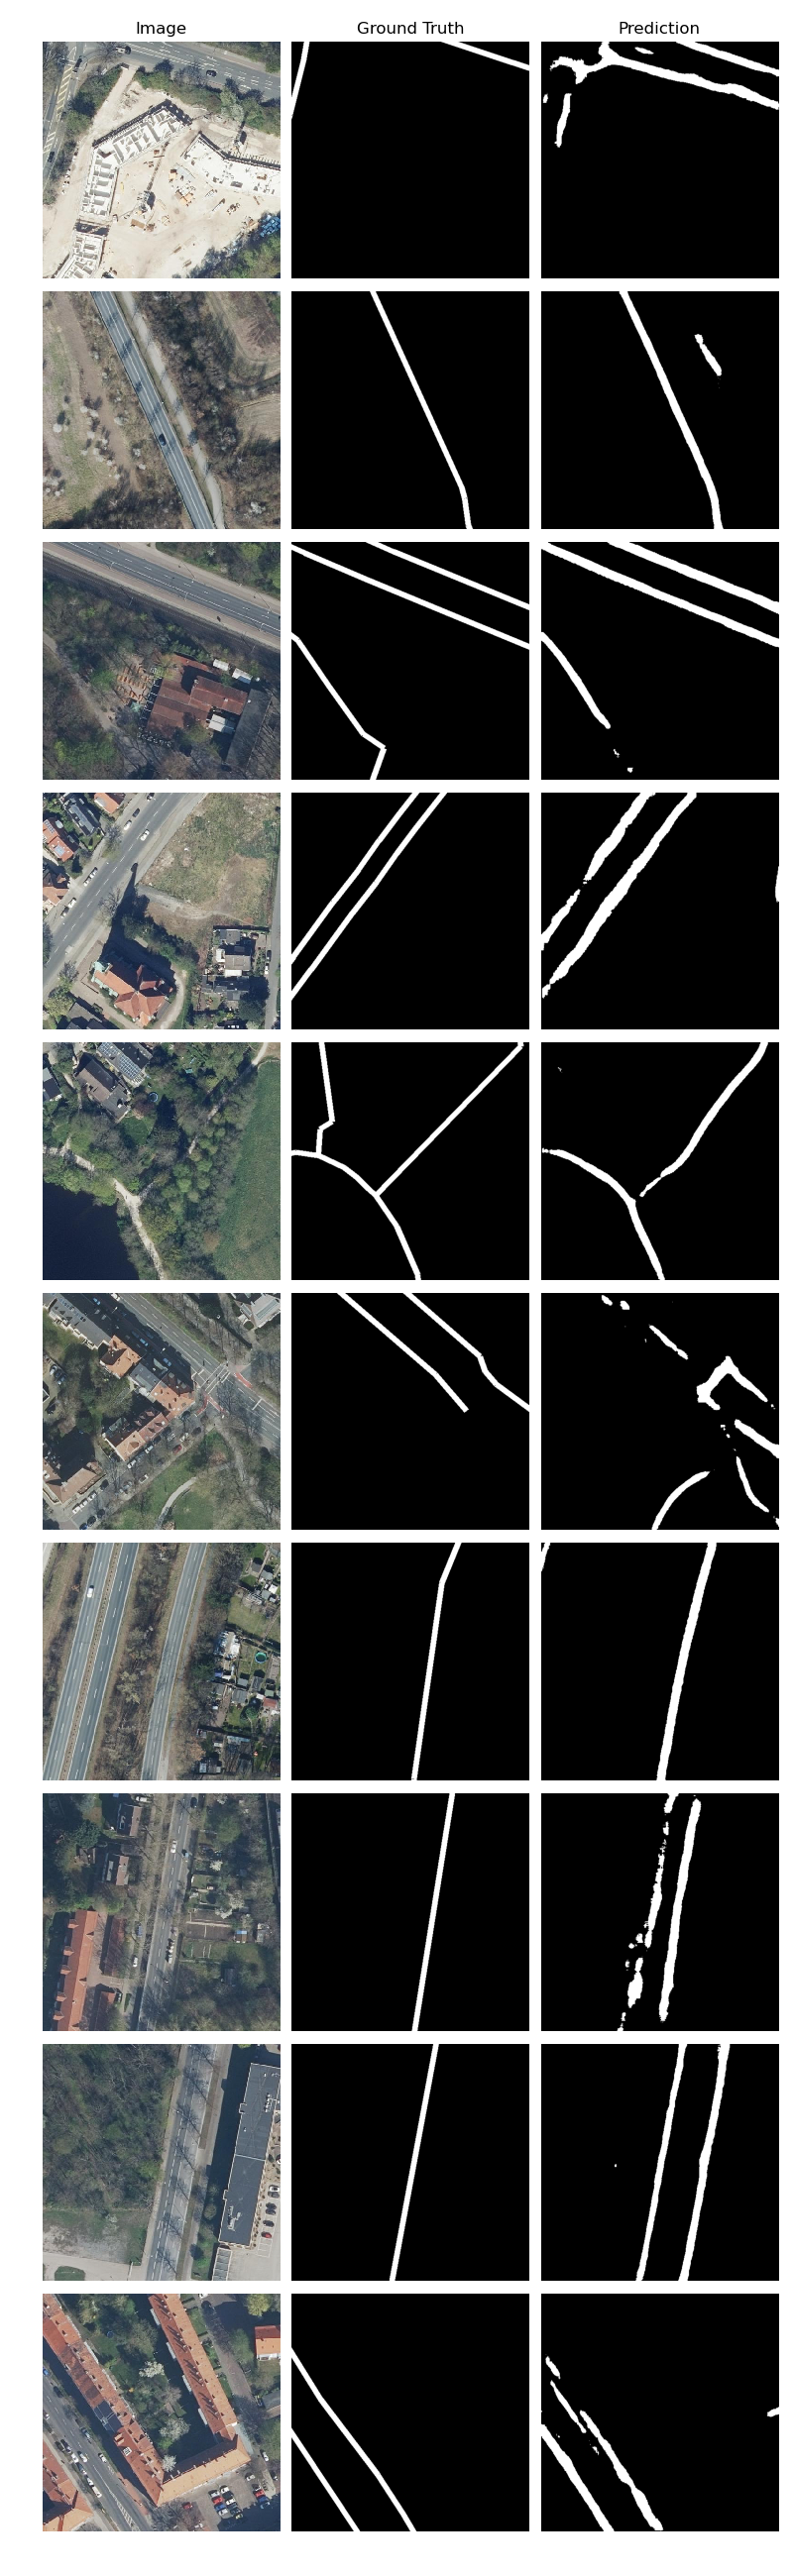
\includegraphics[width=.41\textwidth]{Bilder/Samples-BikeSat/bunet15-l.png} 
	\caption{Beispiel-Predictions des $BUNet15^l$ auf dem BikeSat-Datensatz.}
	\label{fig:bikesat-samples-bunet15-l}
\end{figure}

\begin{figure}
	\centering
	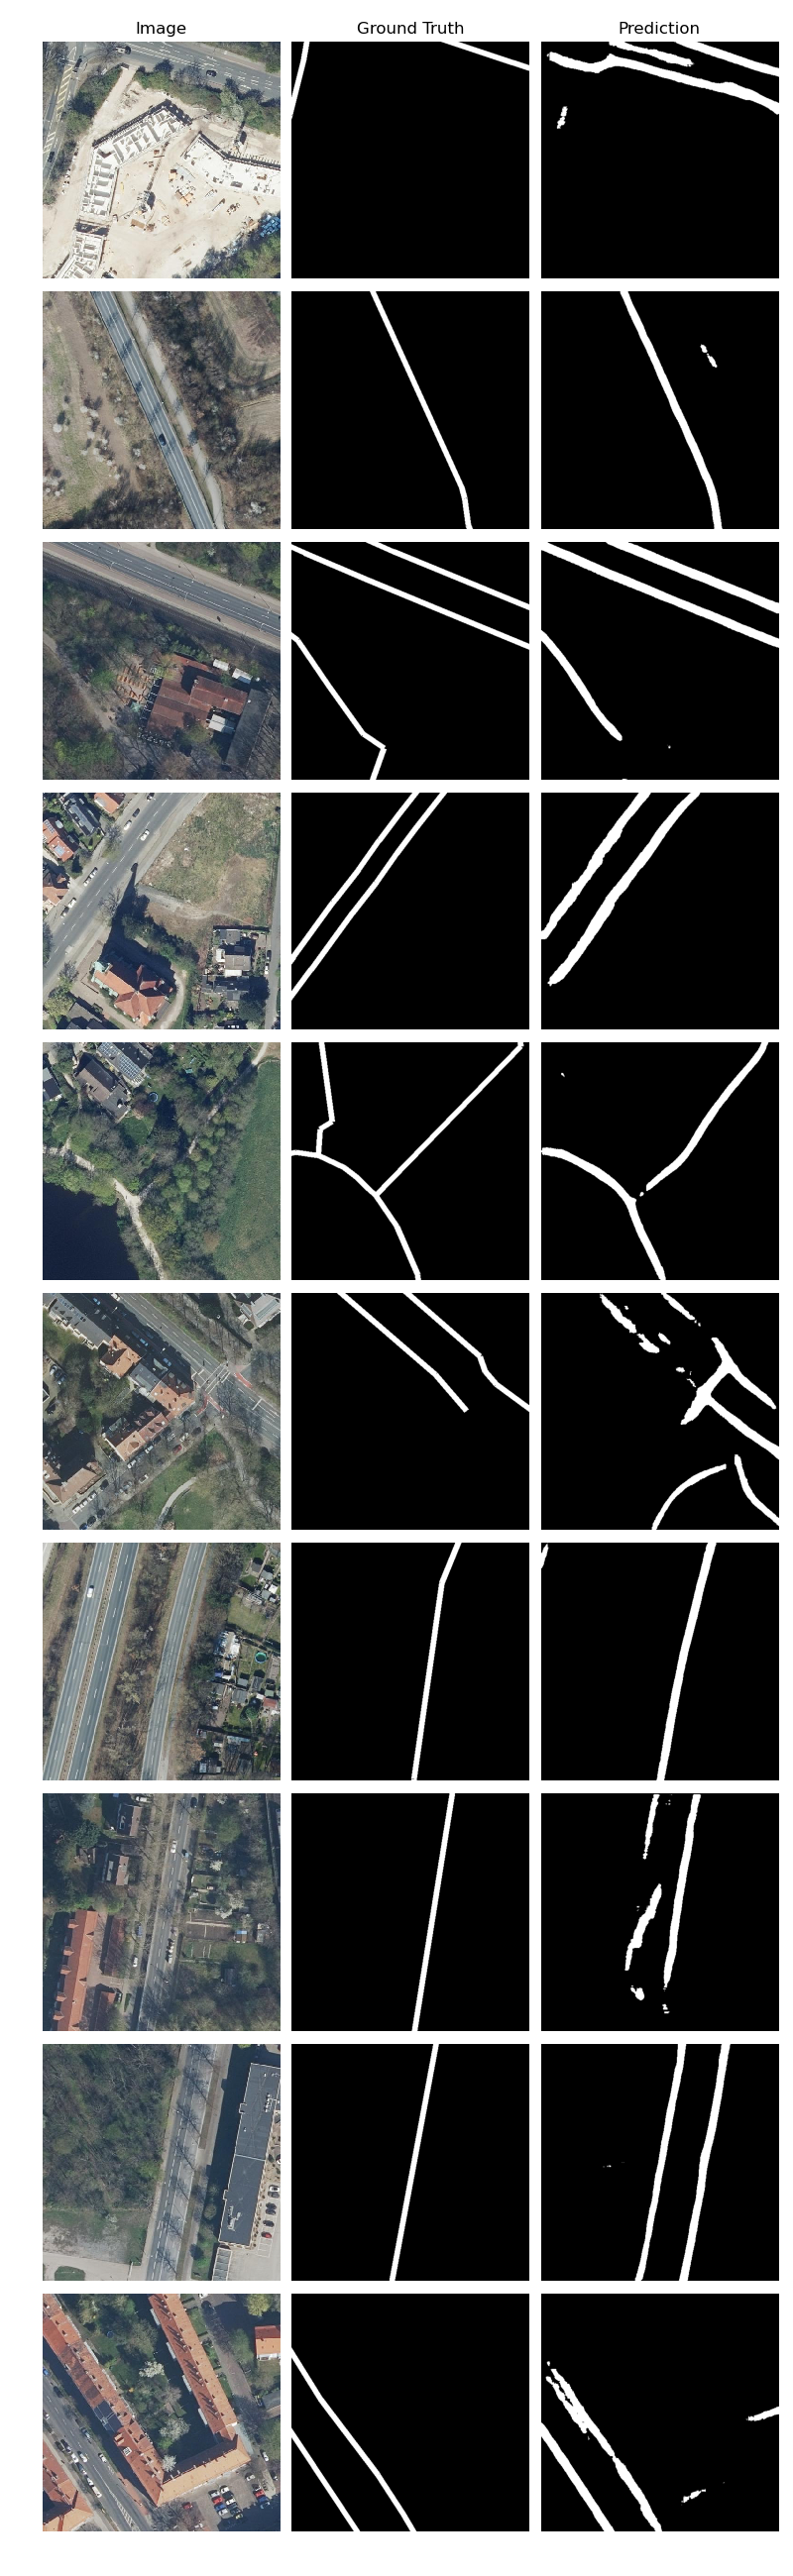
\includegraphics[width=.41\textwidth]{Bilder/Samples-BikeSat/bunet15-r.png} 
	\caption{Beispiel-Predictions des $BUNet15^r$ auf dem BikeSat-Datensatz.}
	\label{fig:bikesat-samples-bunet15-r}
\end{figure}

\begin{figure}
	\centering
	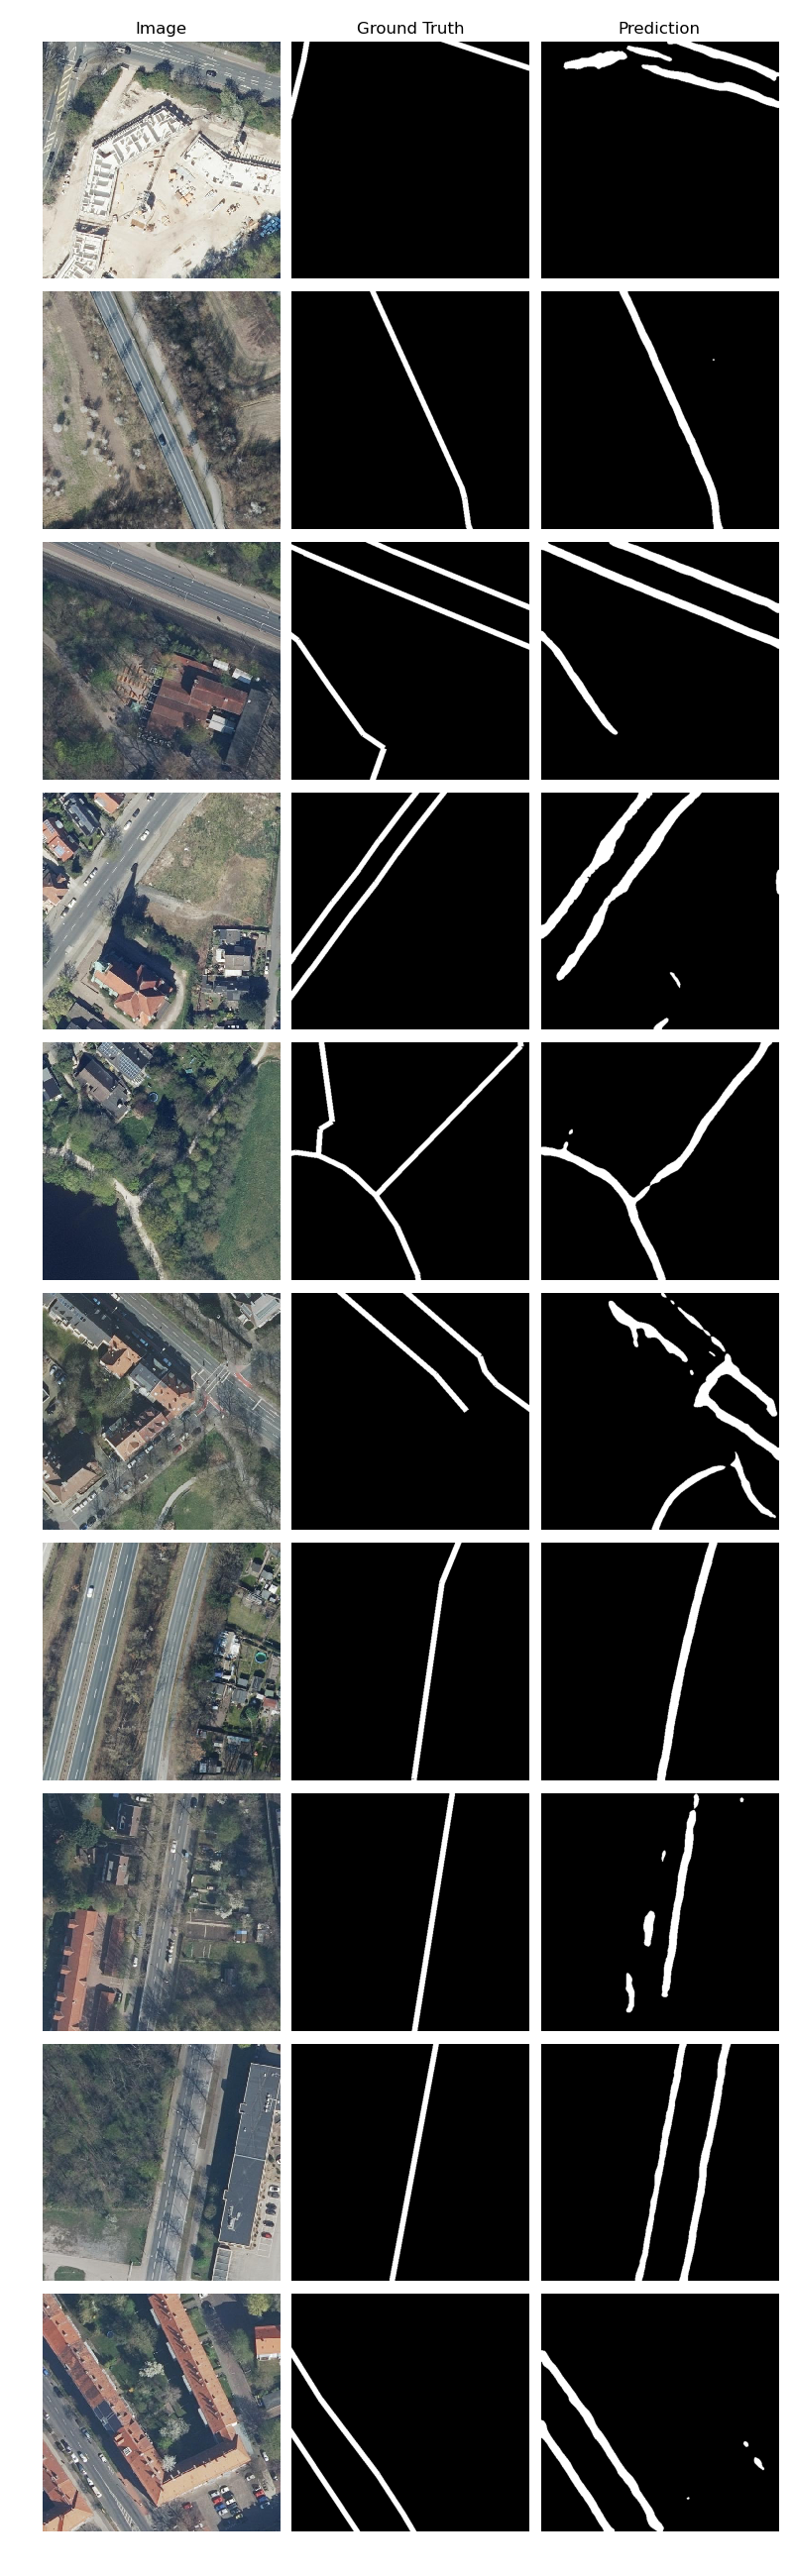
\includegraphics[width=.41\textwidth]{Bilder/Samples-BikeSat/bunet15-s.png} 
	\caption{Beispiel-Predictions des $BUNet15^*$ auf dem BikeSat-Datensatz.}
	\label{fig:bikesat-samples-bunet15-s}
\end{figure}

\begin{figure}
	\centering
	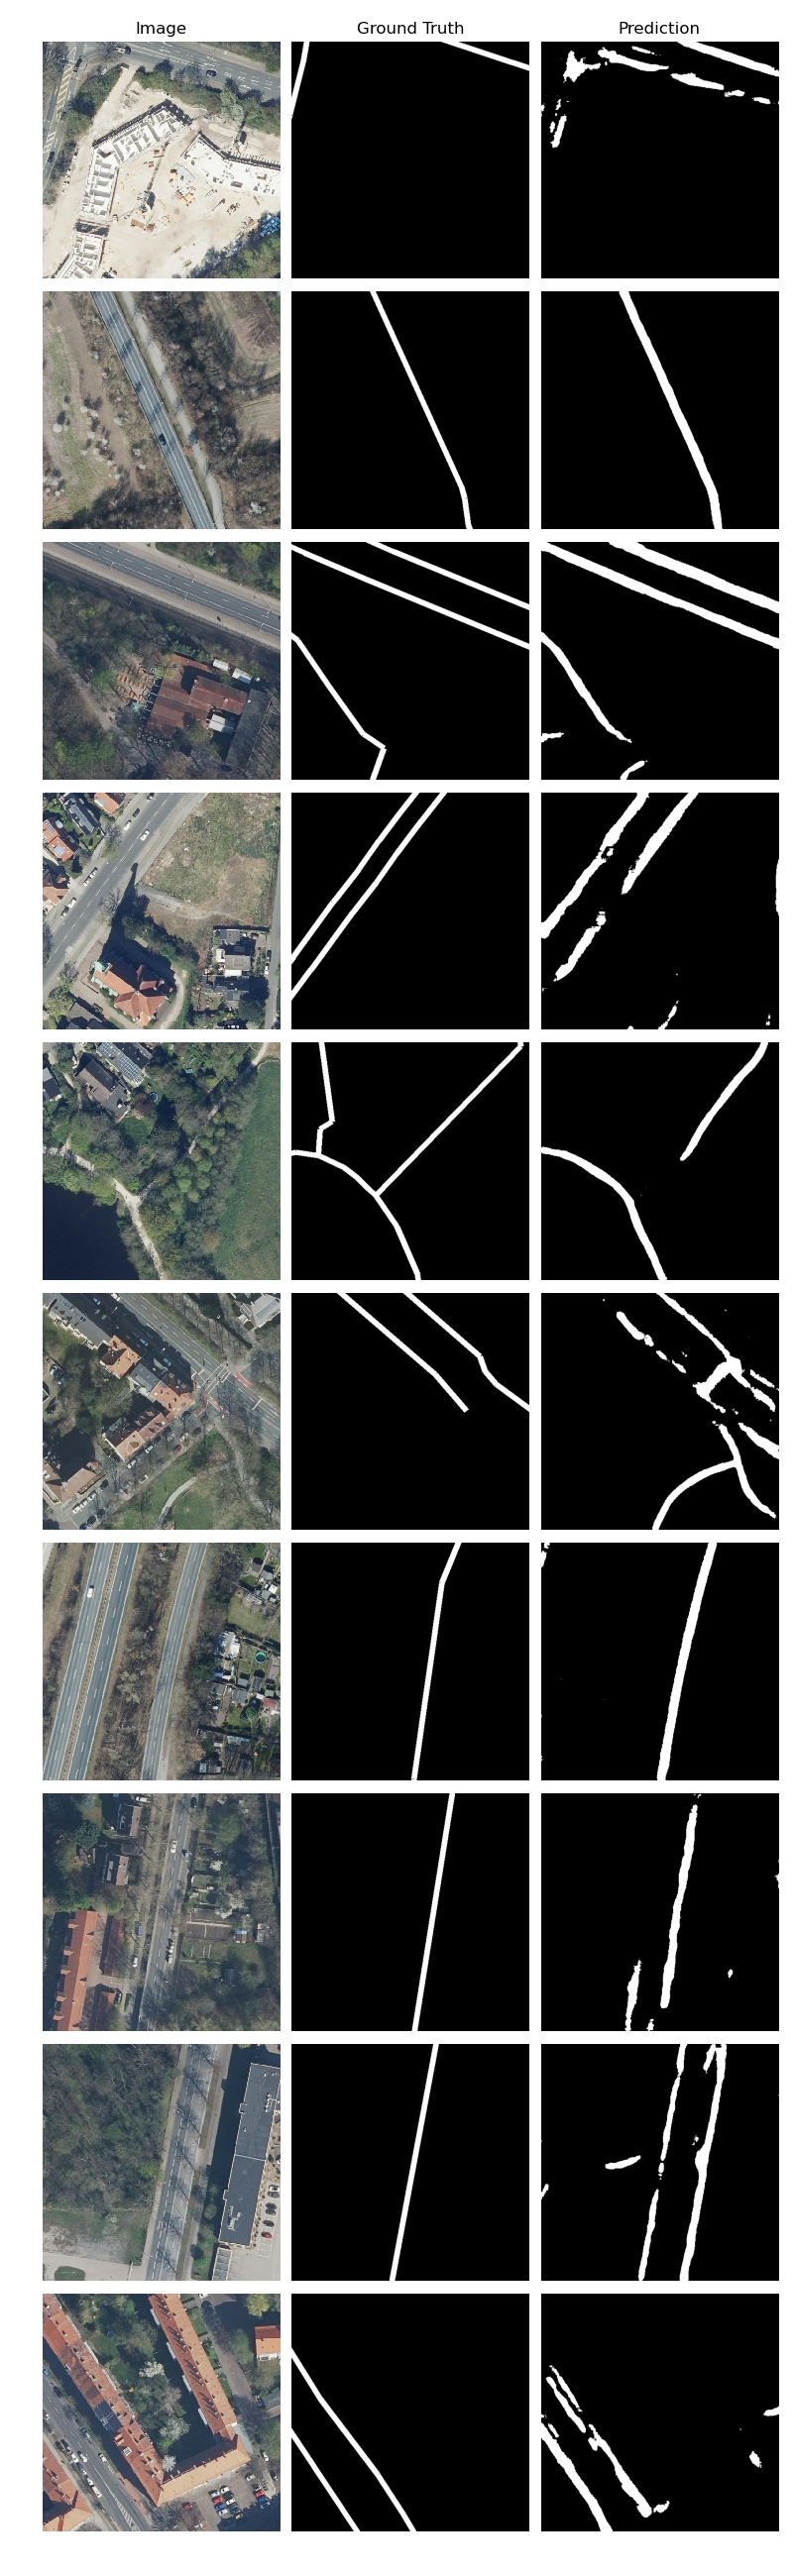
\includegraphics[width=.41\textwidth]{Bilder/Samples-BikeSat/bunet2-l.png} 
	\caption{Beispiel-Predictions des $BUNet2^l$ auf dem BikeSat-Datensatz.}
	\label{fig:bikesat-samples-bunet2-l}
\end{figure}

\begin{figure}
	\centering
	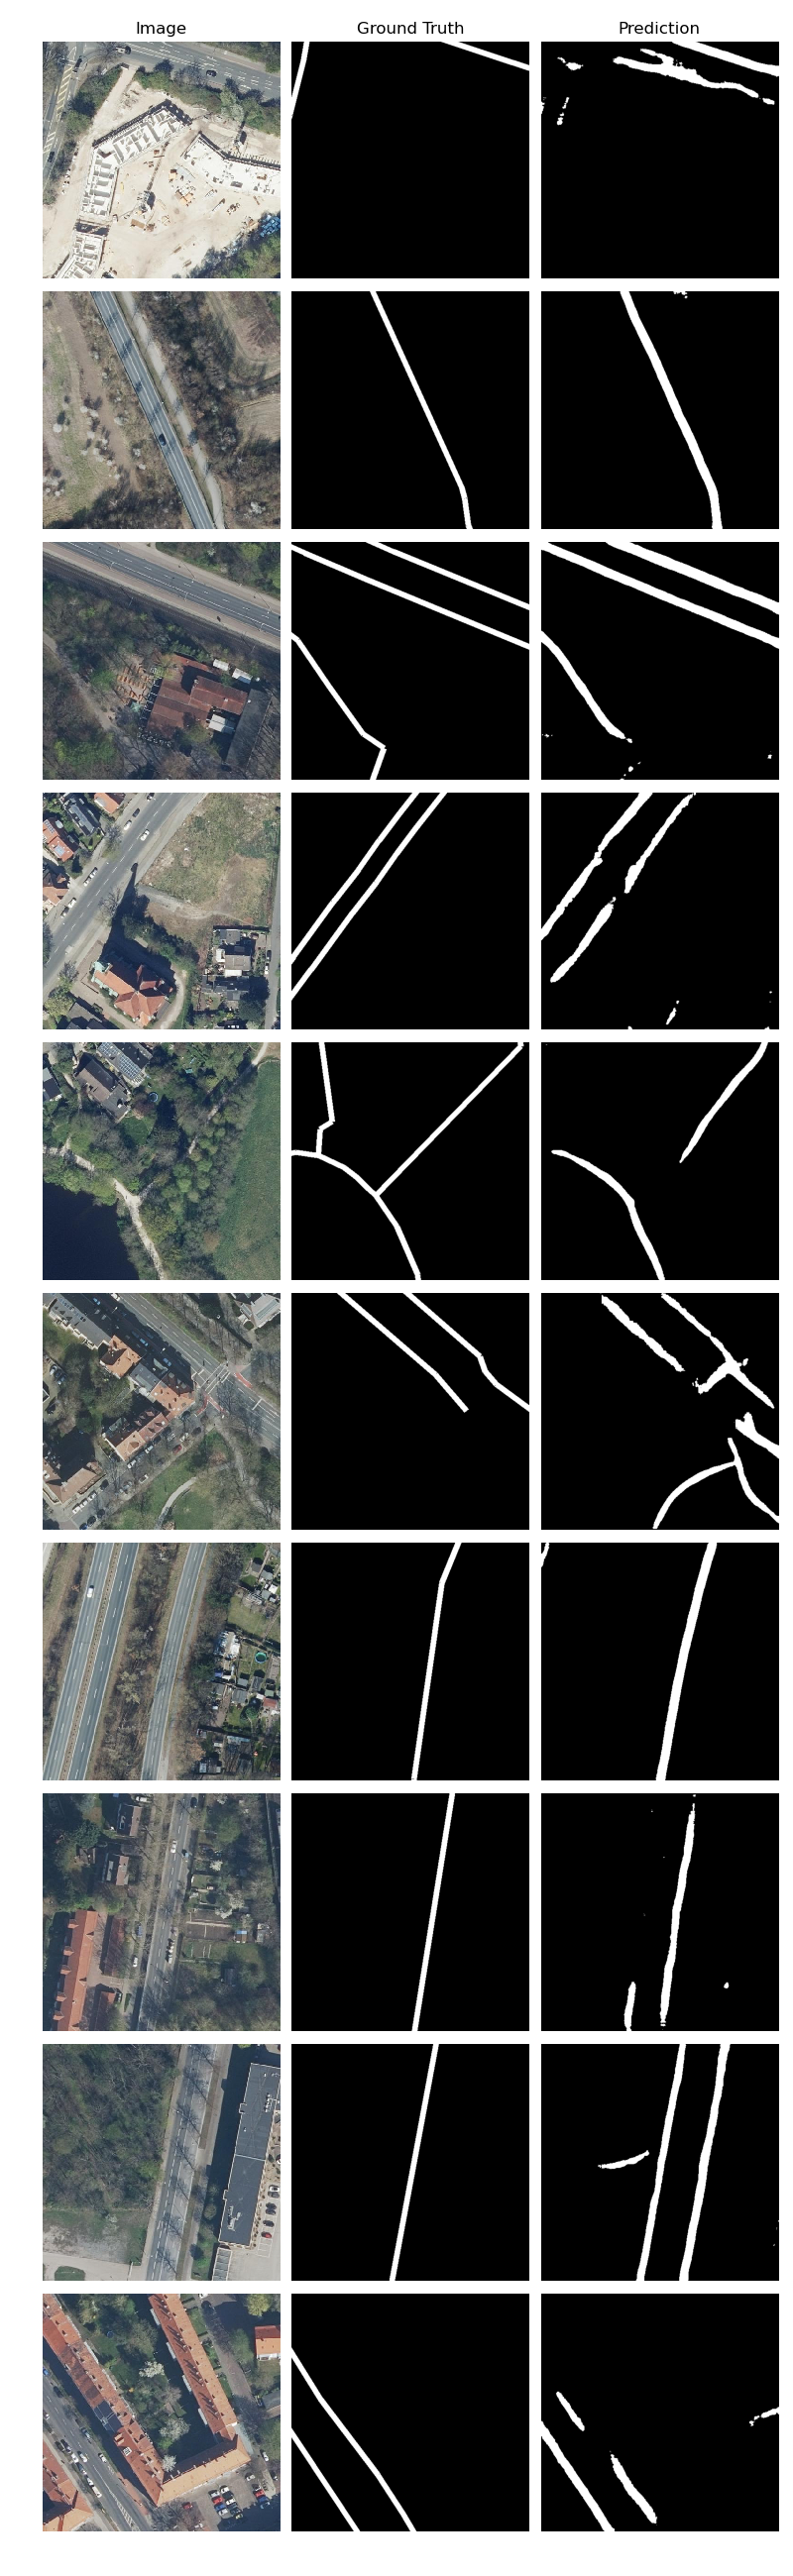
\includegraphics[width=.41\textwidth]{Bilder/Samples-BikeSat/bunet2-r.png} 
	\caption{Beispiel-Predictions des $BUNet2^r$ auf dem BikeSat-Datensatz.}
	\label{fig:bikesat-samples-bunet2-r}
\end{figure}

\begin{figure}
	\centering
	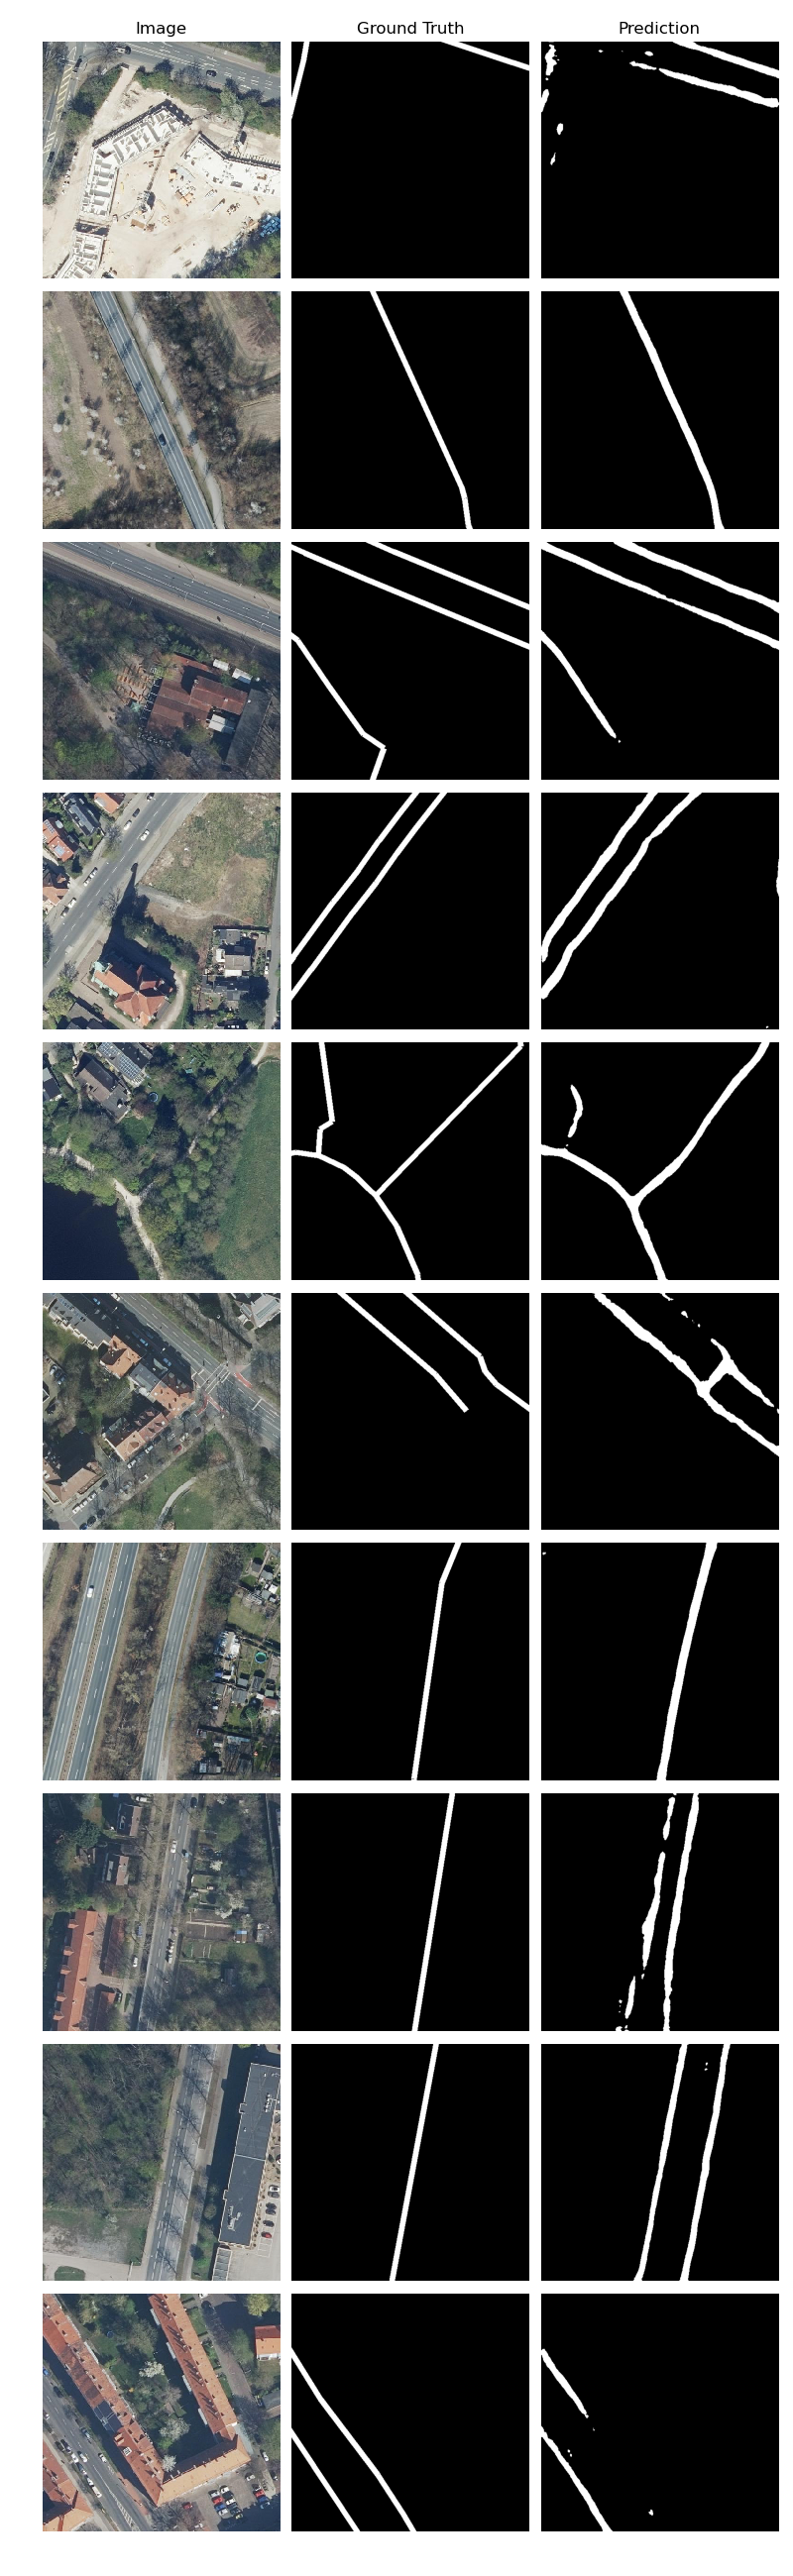
\includegraphics[width=.41\textwidth]{Bilder/Samples-BikeSat/dbunet-l.png} 
	\caption{Beispiel-Predictions des $DBUNet^l$ auf dem BikeSat-Datensatz.}
	\label{fig:bikesat-samples-dbunet-l}
\end{figure}

\begin{figure}
	\centering
	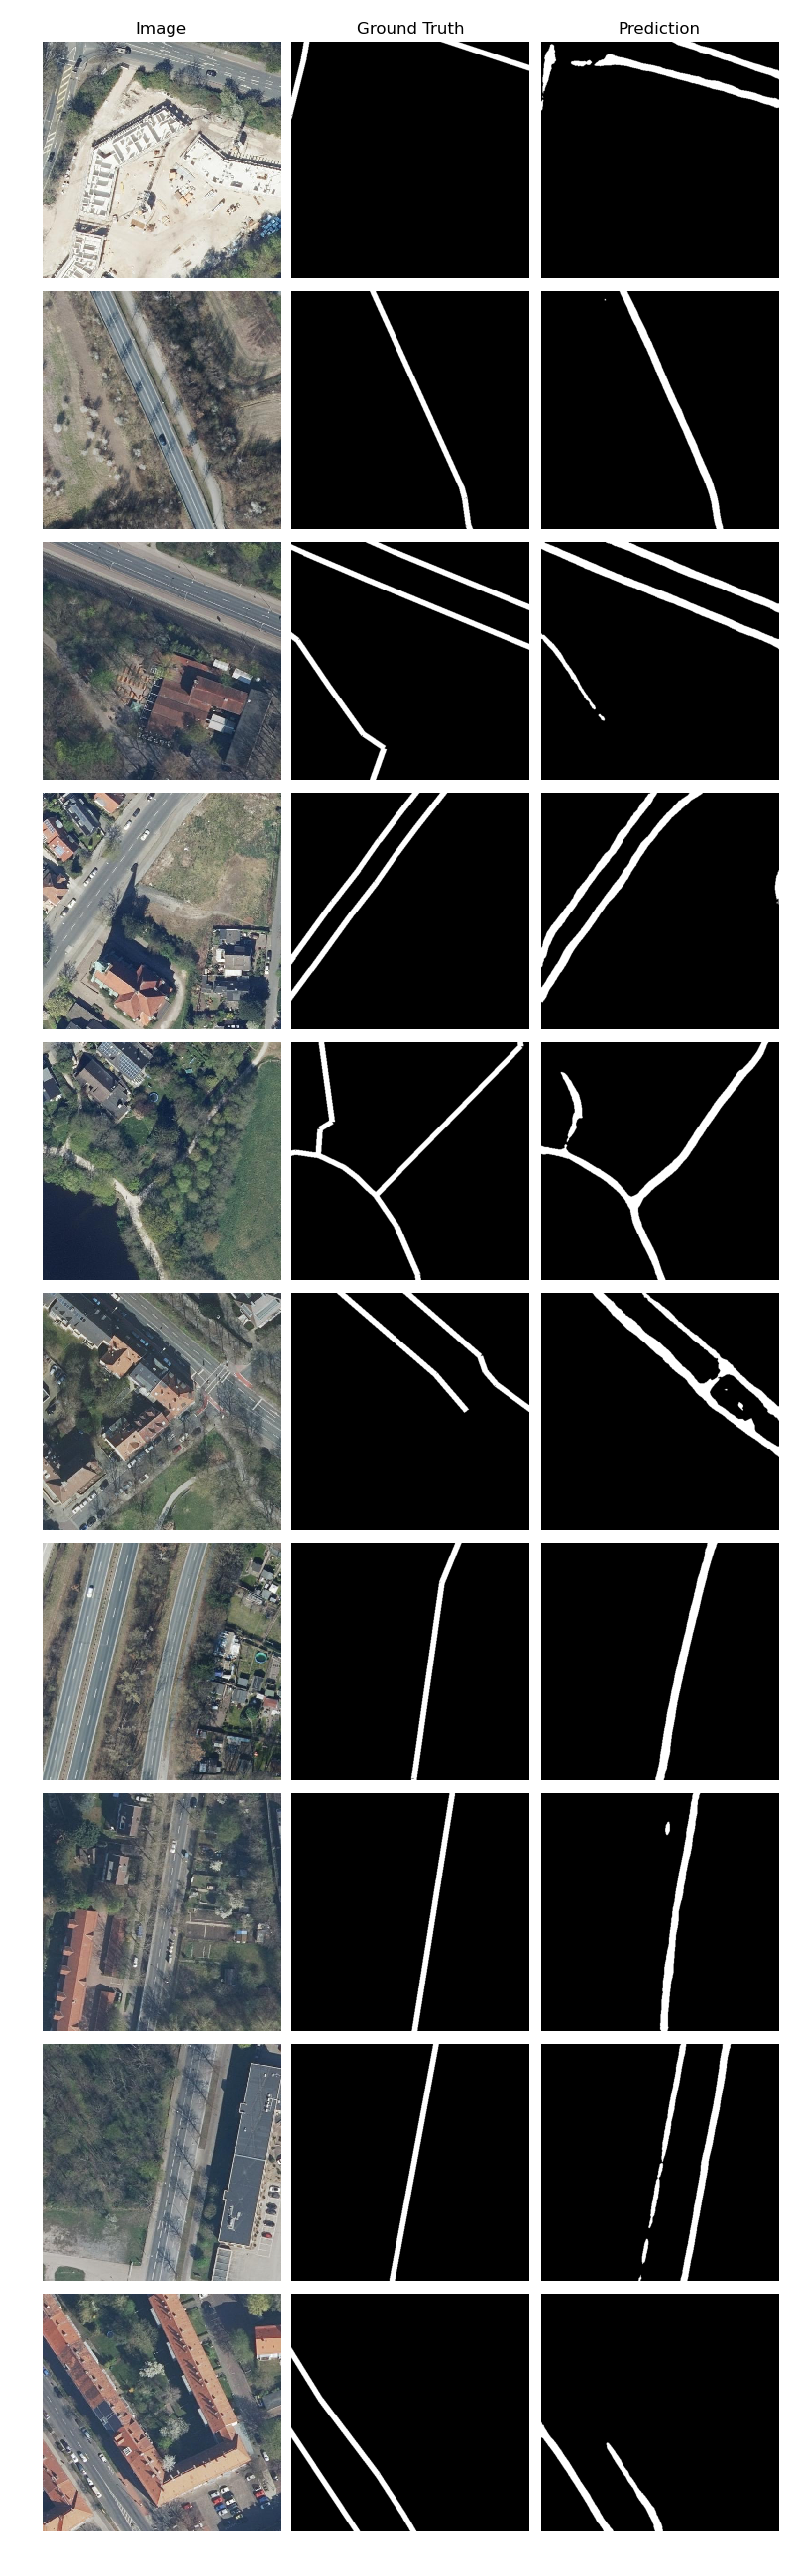
\includegraphics[width=.41\textwidth]{Bilder/Samples-BikeSat/dbunet-r.png} 
	\caption{Beispiel-Predictions des $DBUNet^r$ auf dem BikeSat-Datensatz.}
	\label{fig:bikesat-samples-dbunet-r}
\end{figure}

\begin{figure}
	\centering
	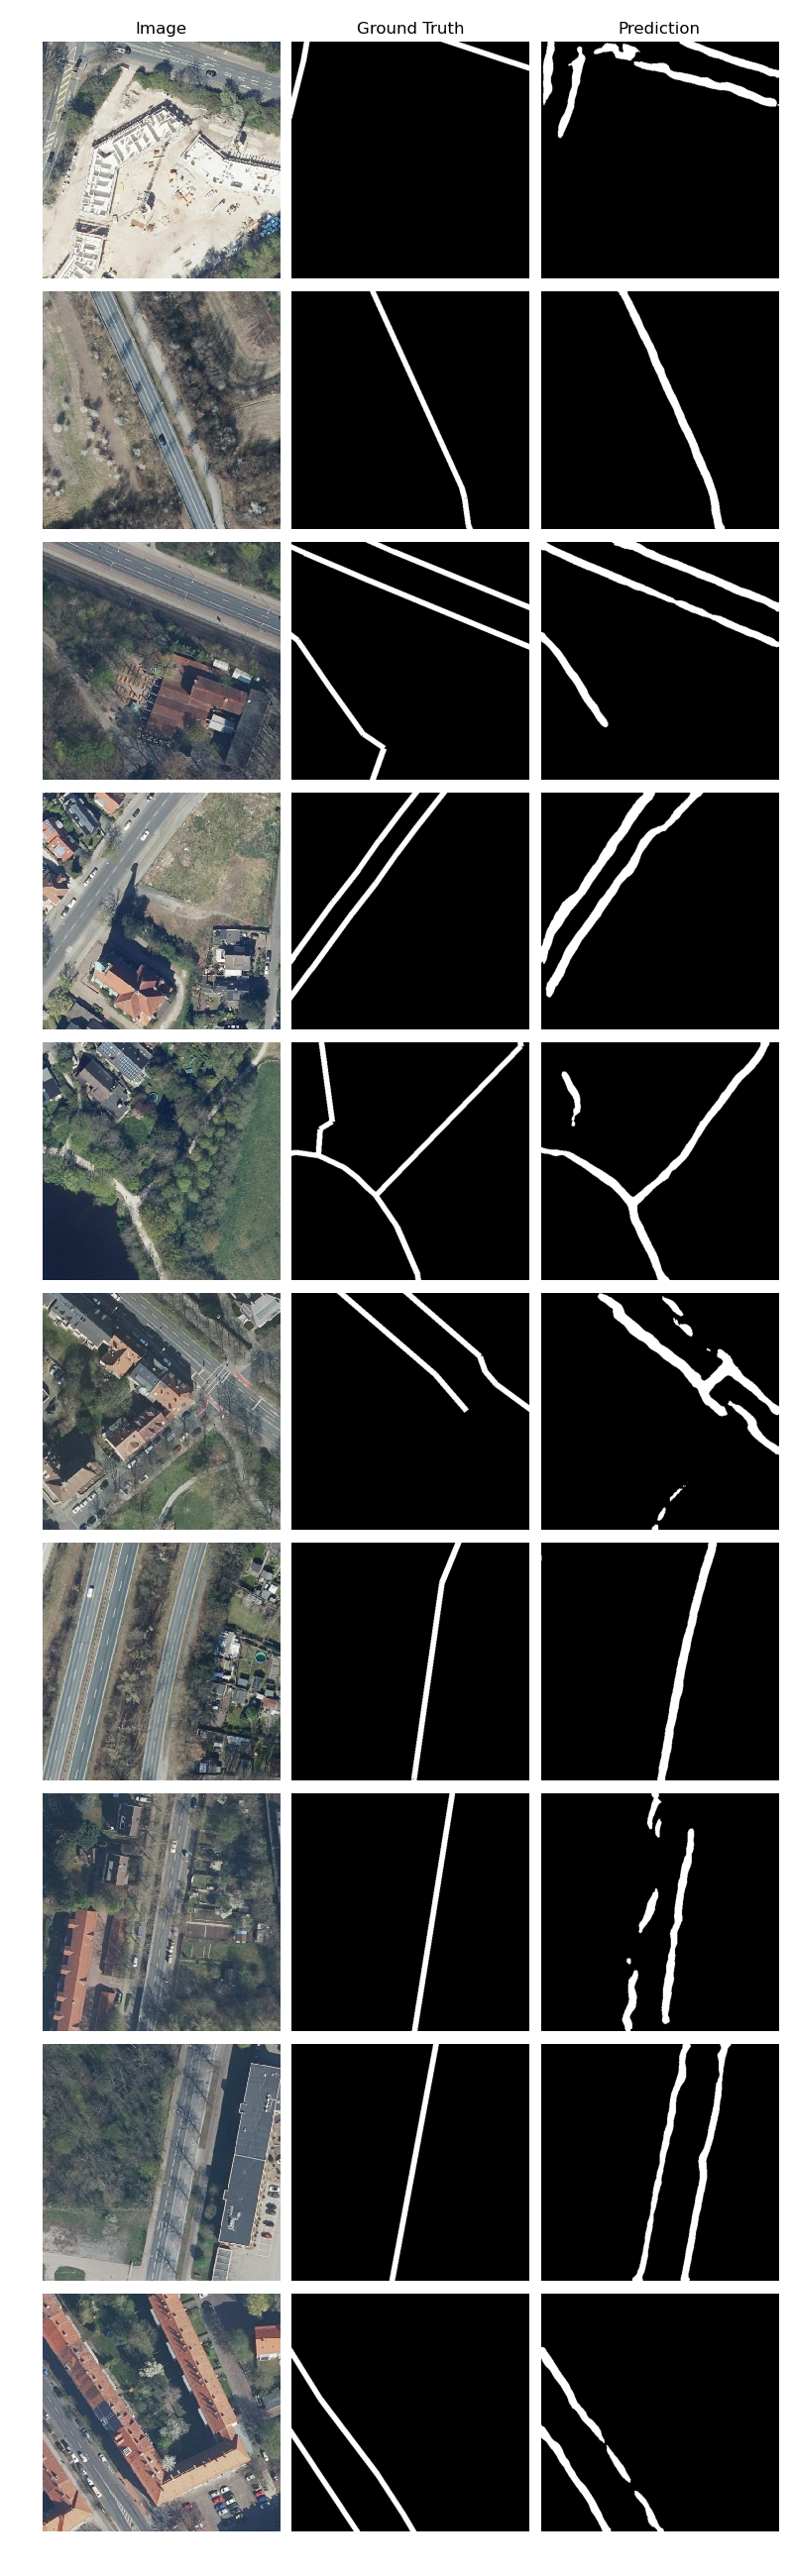
\includegraphics[width=.41\textwidth]{Bilder/Samples-BikeSat/dbunet-s.png} 
	\caption{Beispiel-Predictions des $DBUNet^*$ auf dem BikeSat-Datensatz.}
	\label{fig:bikesat-samples-dbunet-s}
\end{figure}

\begin{figure}
	\centering
	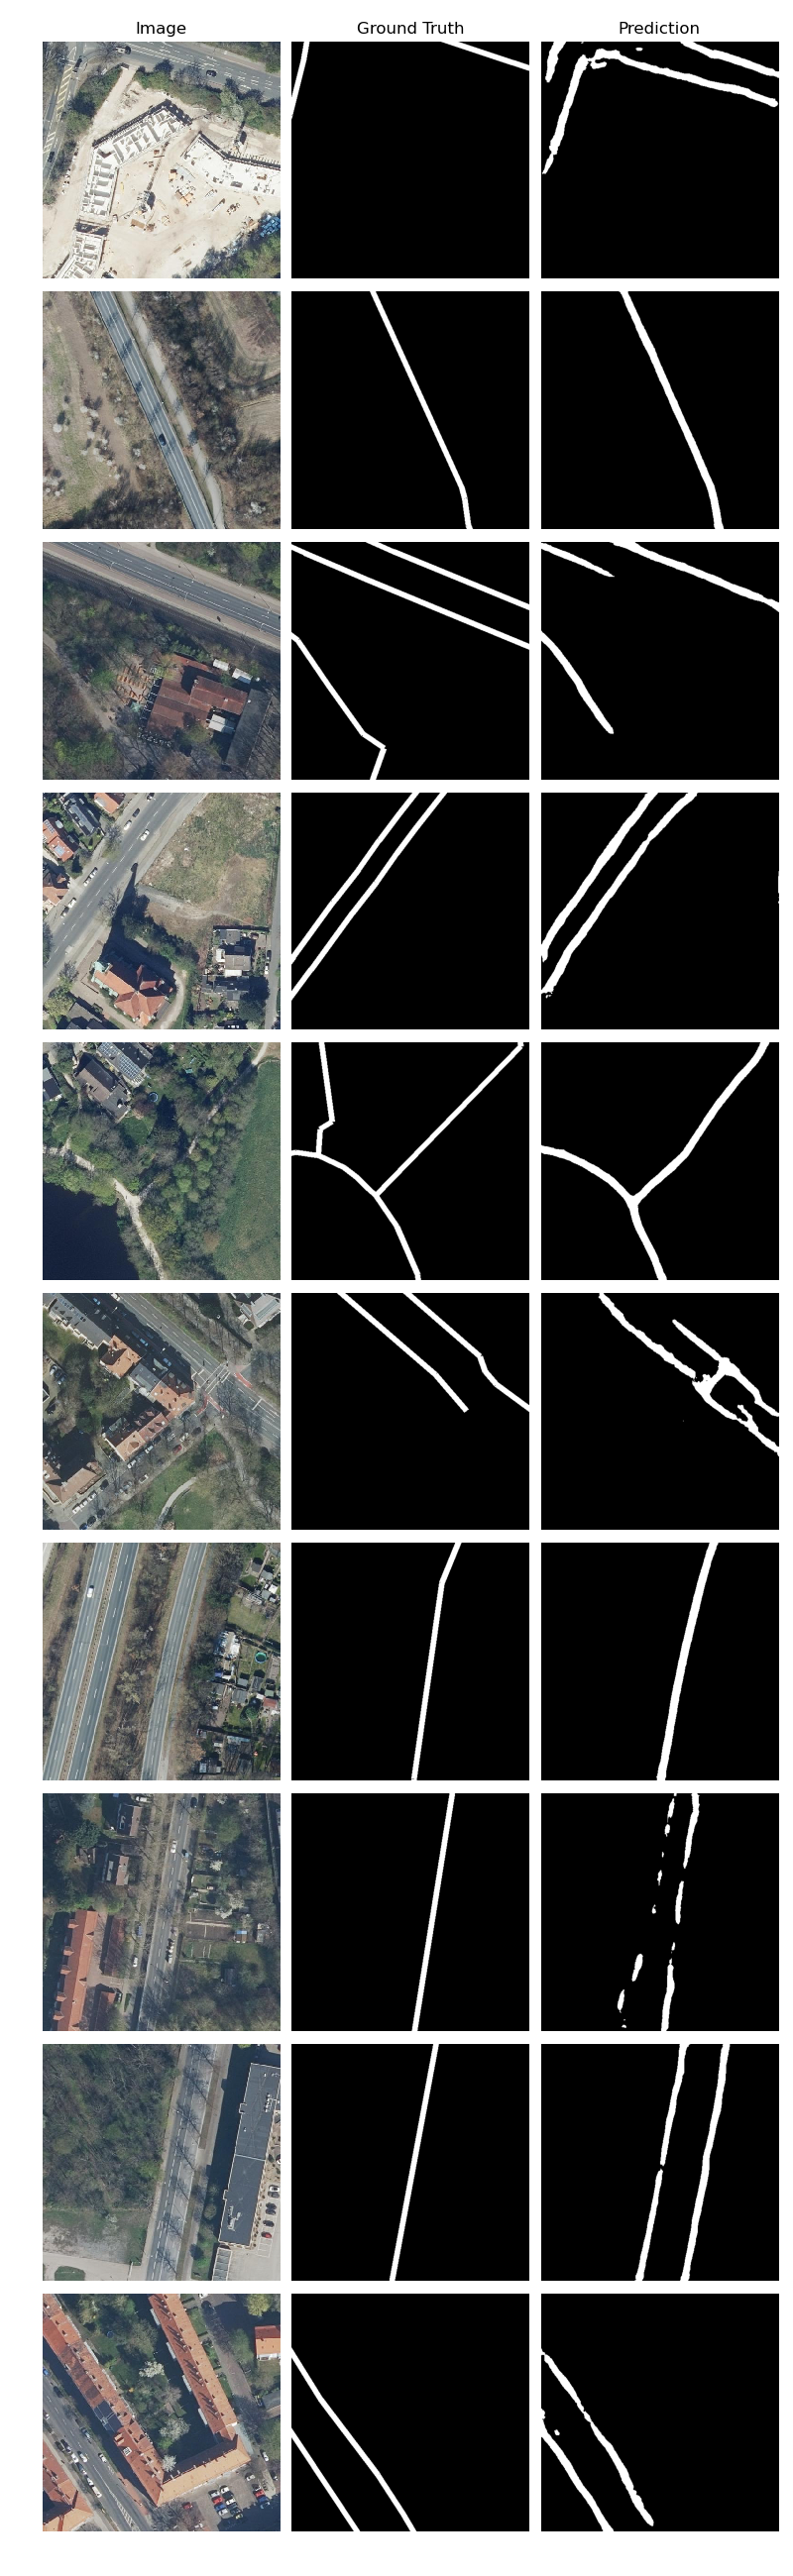
\includegraphics[width=.41\textwidth]{Bilder/Samples-BikeSat/rbunet-l.png} 
	\caption{Beispiel-Predictions des $RBUNet^l$ auf dem BikeSat-Datensatz.}
	\label{fig:bikesat-samples-rbunet-l}
\end{figure}

\begin{figure}
	\centering
	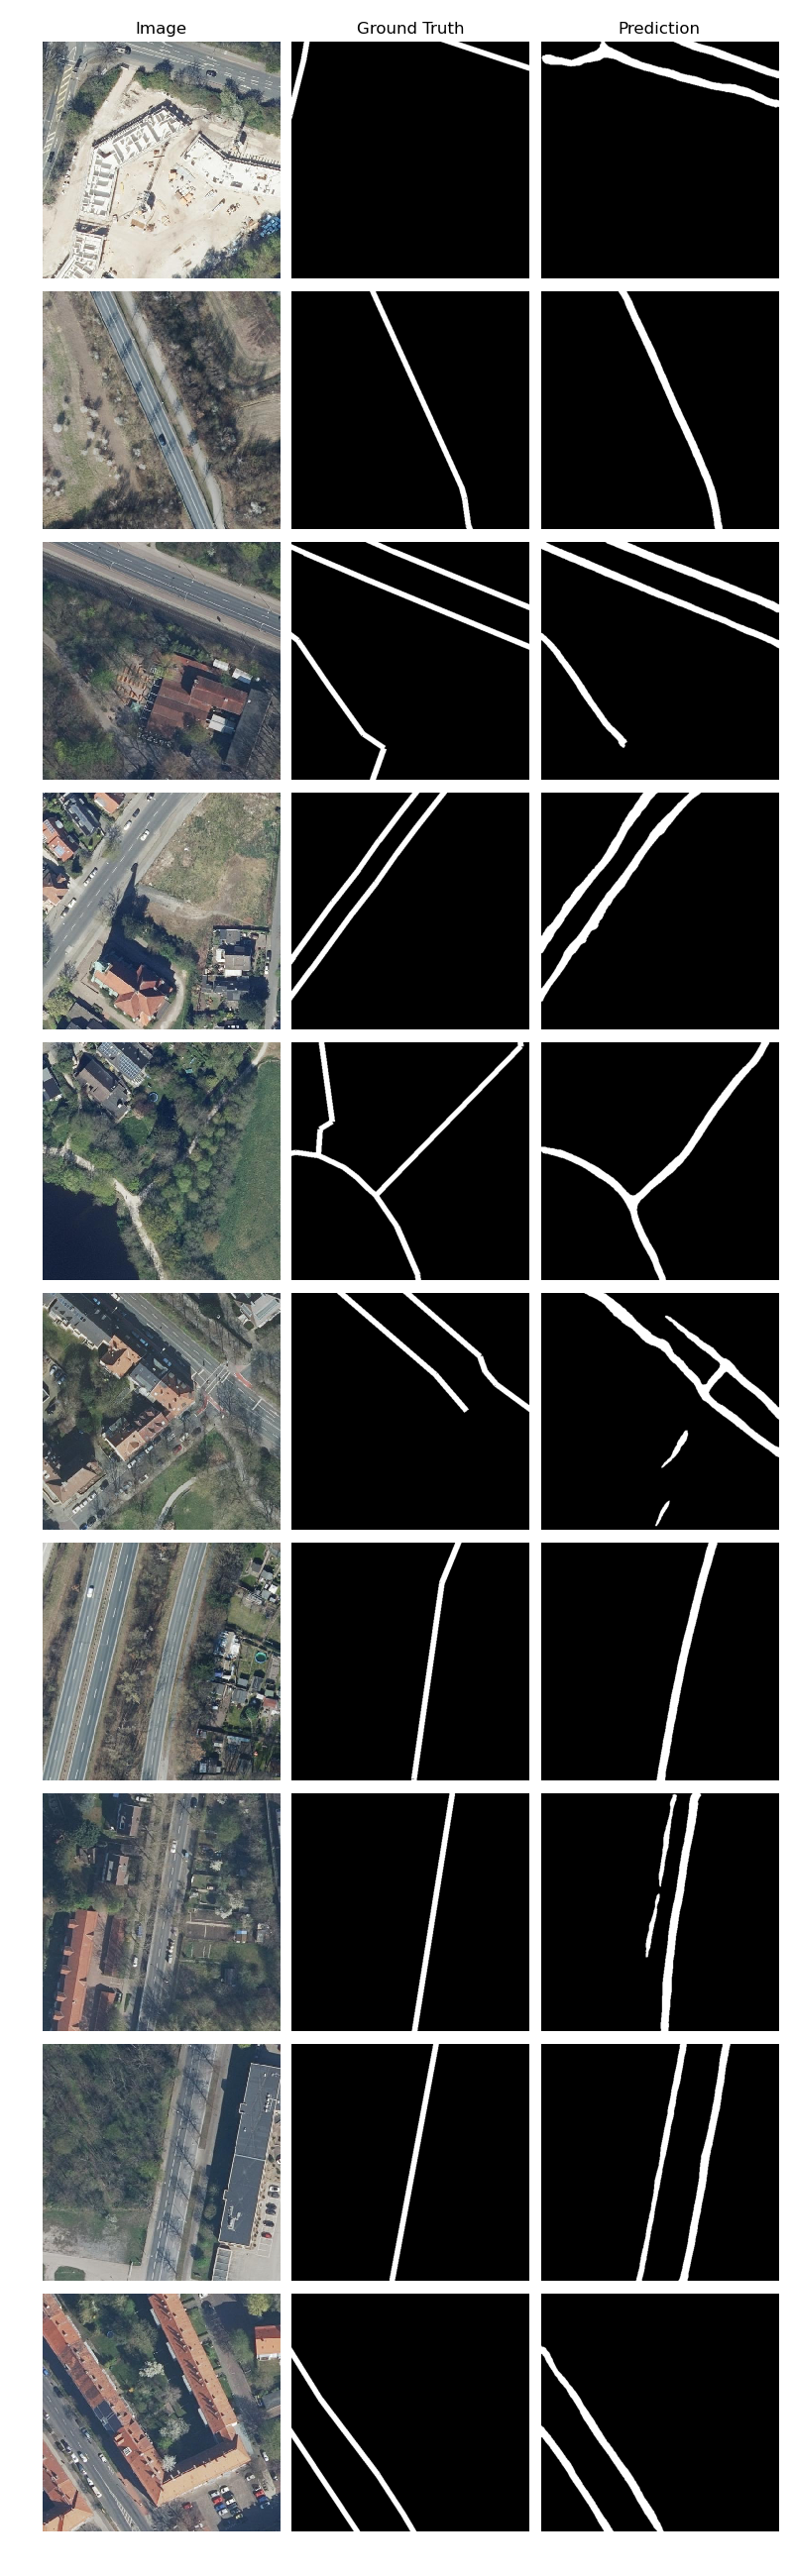
\includegraphics[width=.41\textwidth]{Bilder/Samples-BikeSat/rbunet-r.png} 
	\caption{Beispiel-Predictions des $RBUNet^r$ auf dem BikeSat-Datensatz.}
	\label{fig:bikesat-samples-rbunet-r}
\end{figure}

\begin{figure}
	\centering
	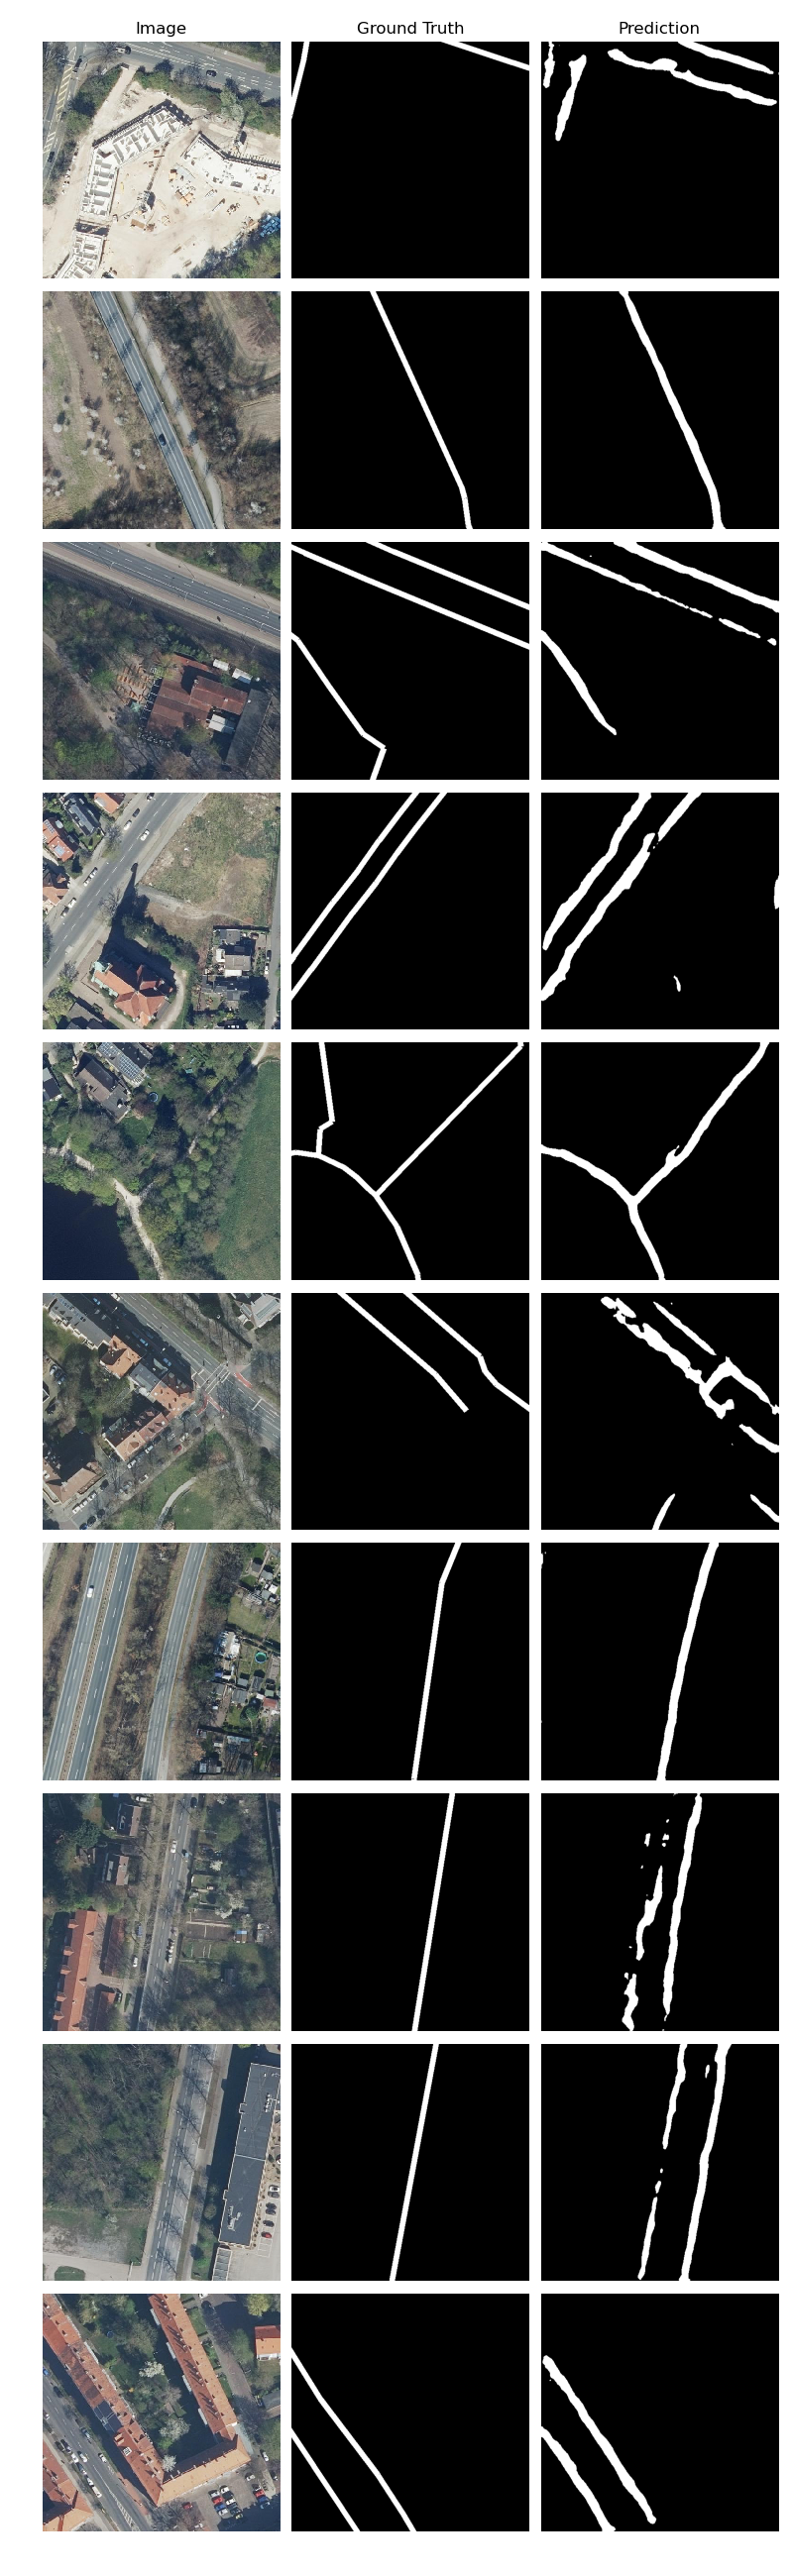
\includegraphics[width=.41\textwidth]{Bilder/Samples-BikeSat/rbunet-s.png} 
	\caption{Beispiel-Predictions des $RBUNet^*$ auf dem BikeSat-Datensatz.}
	\label{fig:bikesat-samples-rbunet-s}
\end{figure}

\begin{figure}
	\centering
	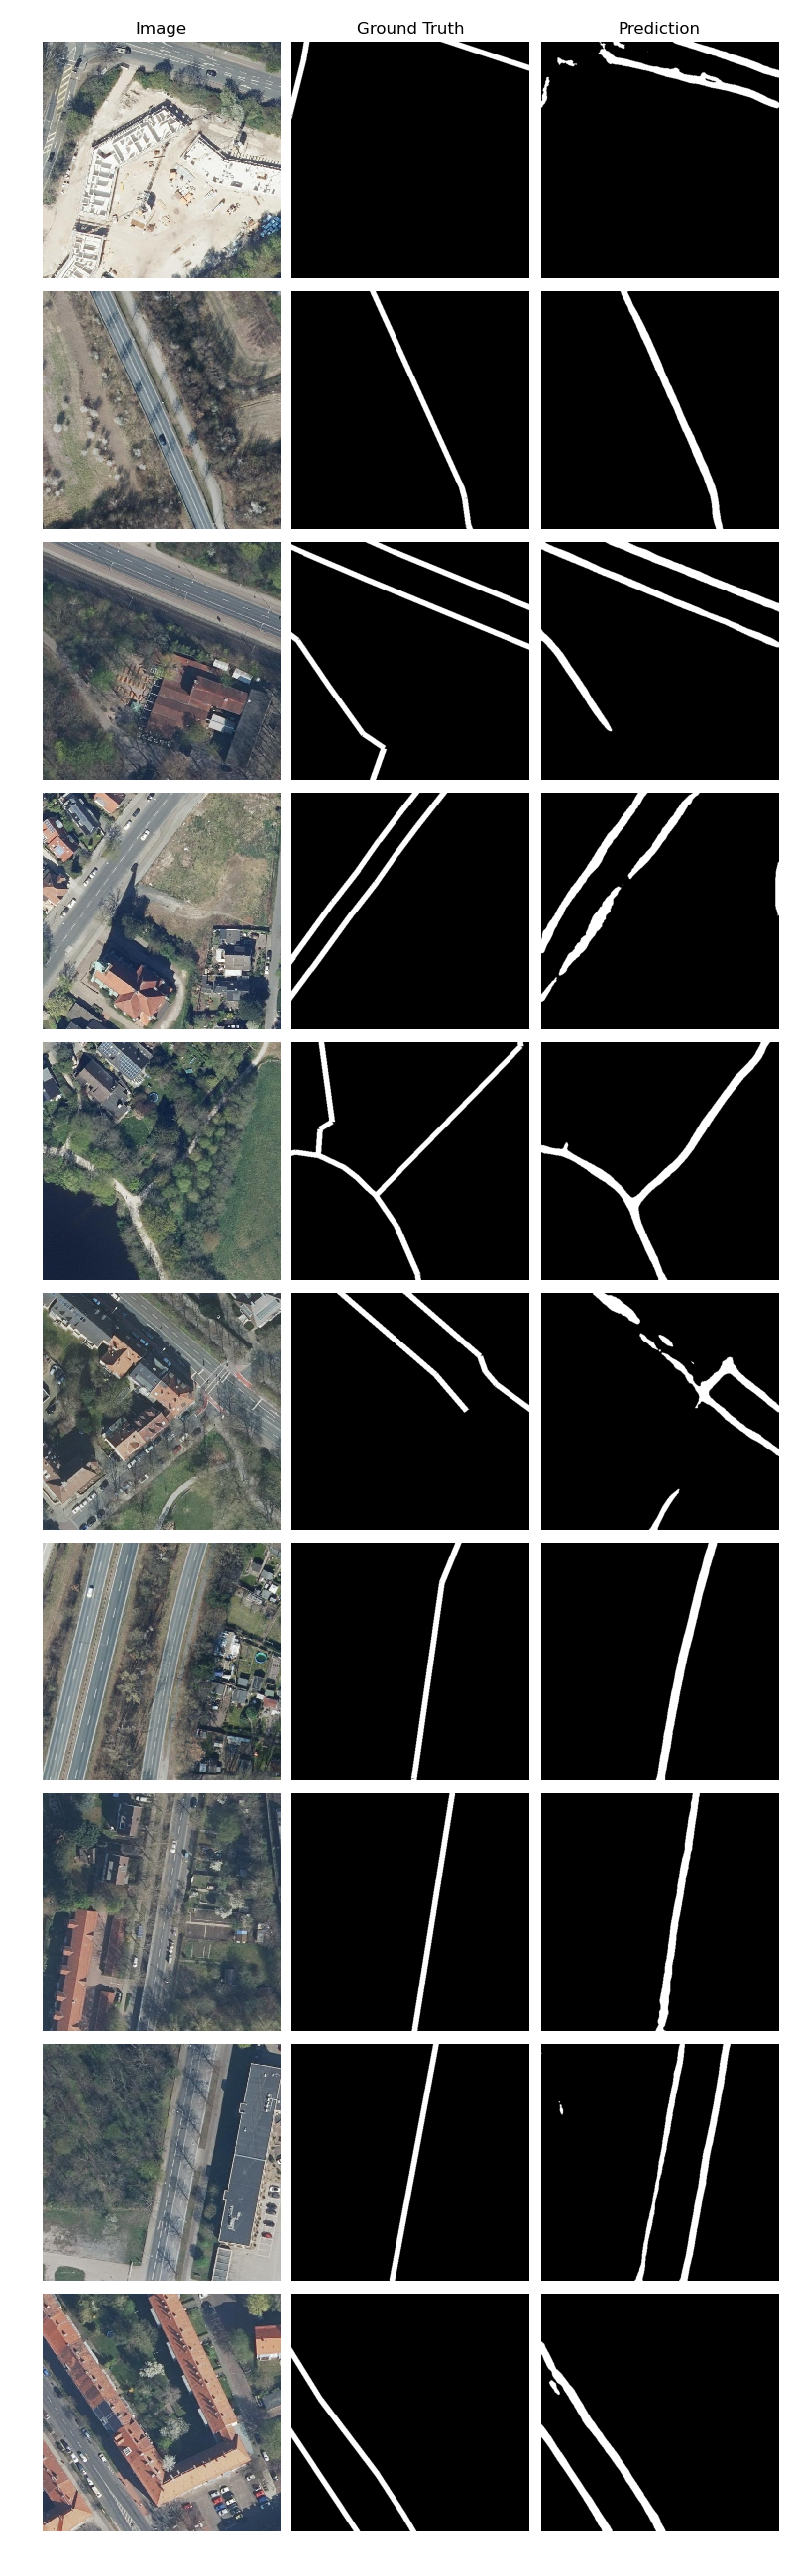
\includegraphics[width=.41\textwidth]{Bilder/Samples-BikeSat/vbunet-r.png} 
	\caption{Beispiel-Predictions des $VBUNet^r$ auf dem BikeSat-Datensatz.}
	\label{fig:bikesat-samples-vbunet-r}
\end{figure}

\begin{figure}
	\centering
	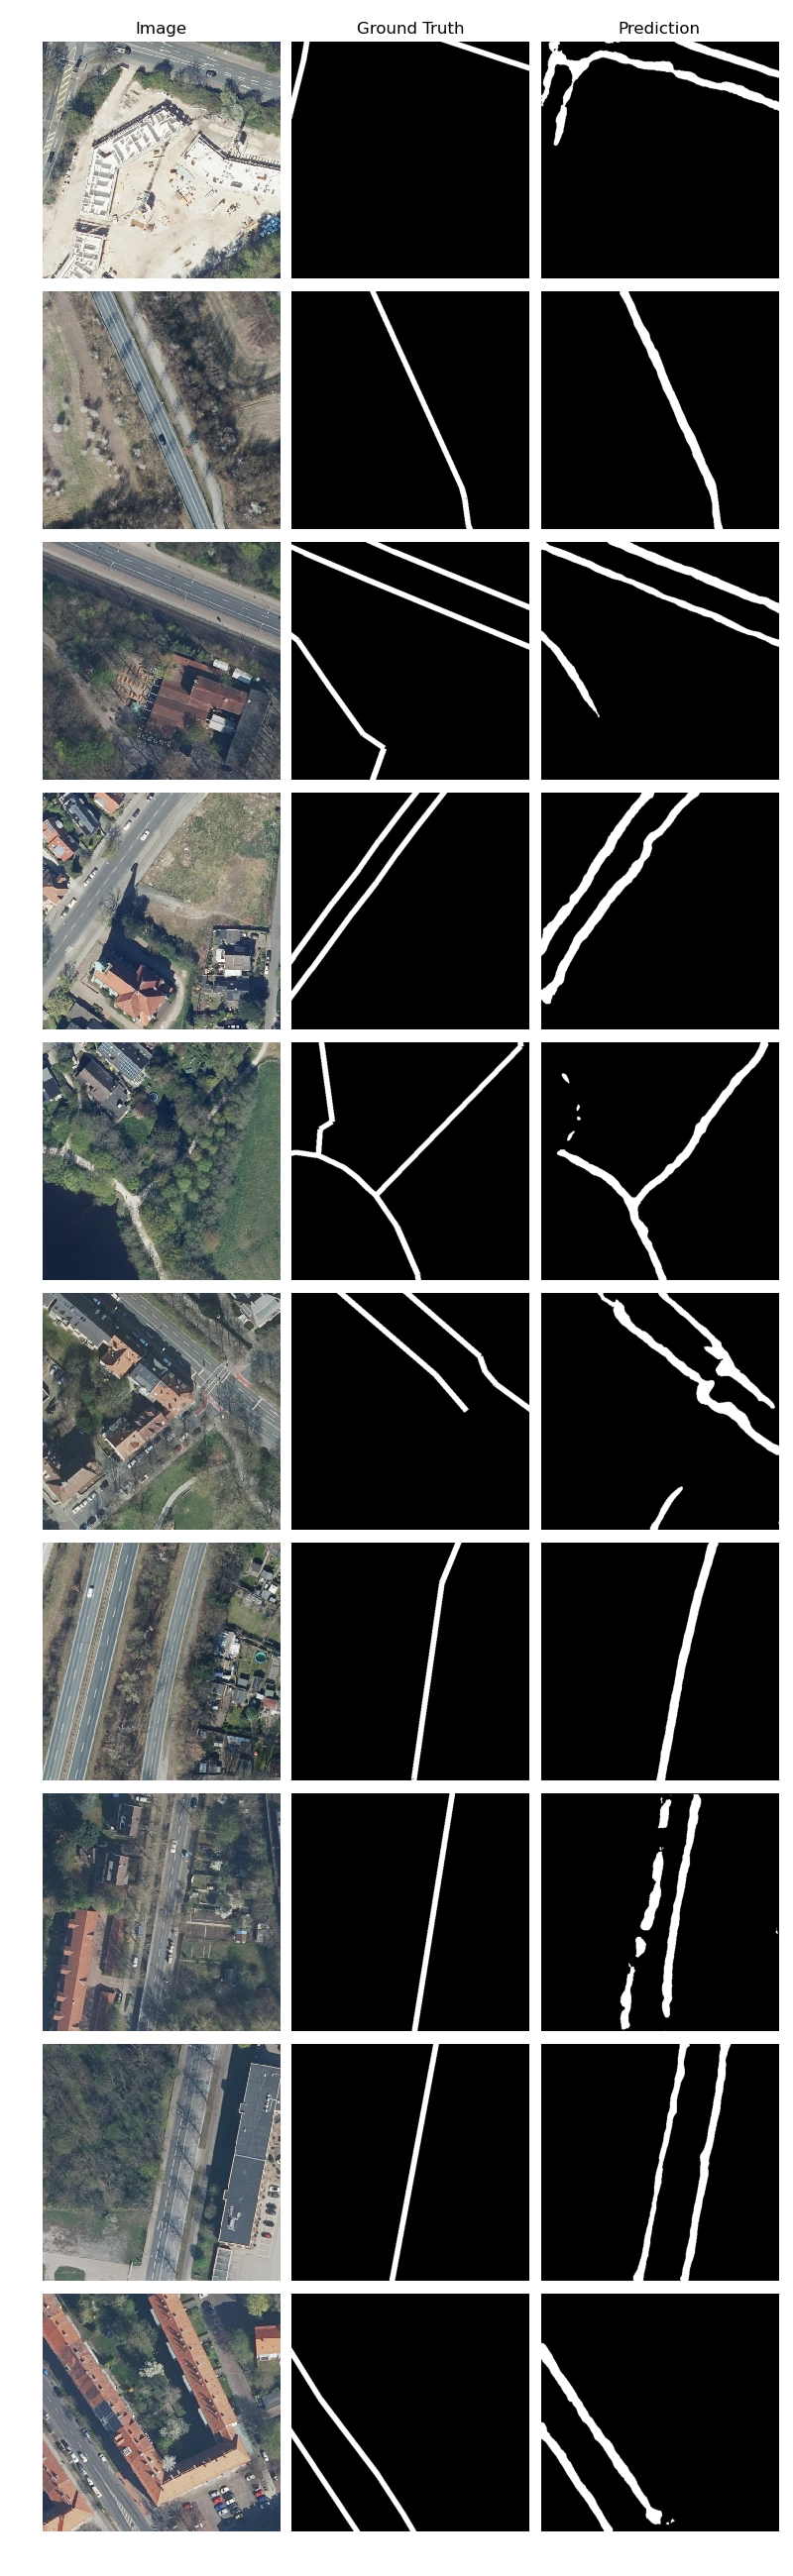
\includegraphics[width=.41\textwidth]{Bilder/Samples-BikeSat/vbunet-s.png} 
	\caption{Beispiel-Predictions des $VBUNet^*$ auf dem BikeSat-Datensatz.}
	\label{fig:bikesat-samples-vbunet-s}
\end{figure}

\pagebreak 


\section{Beispiel-Predictions Karlsruhe} \label{sec:pred-karlsruhe}

\begin{figure}
	\centering
	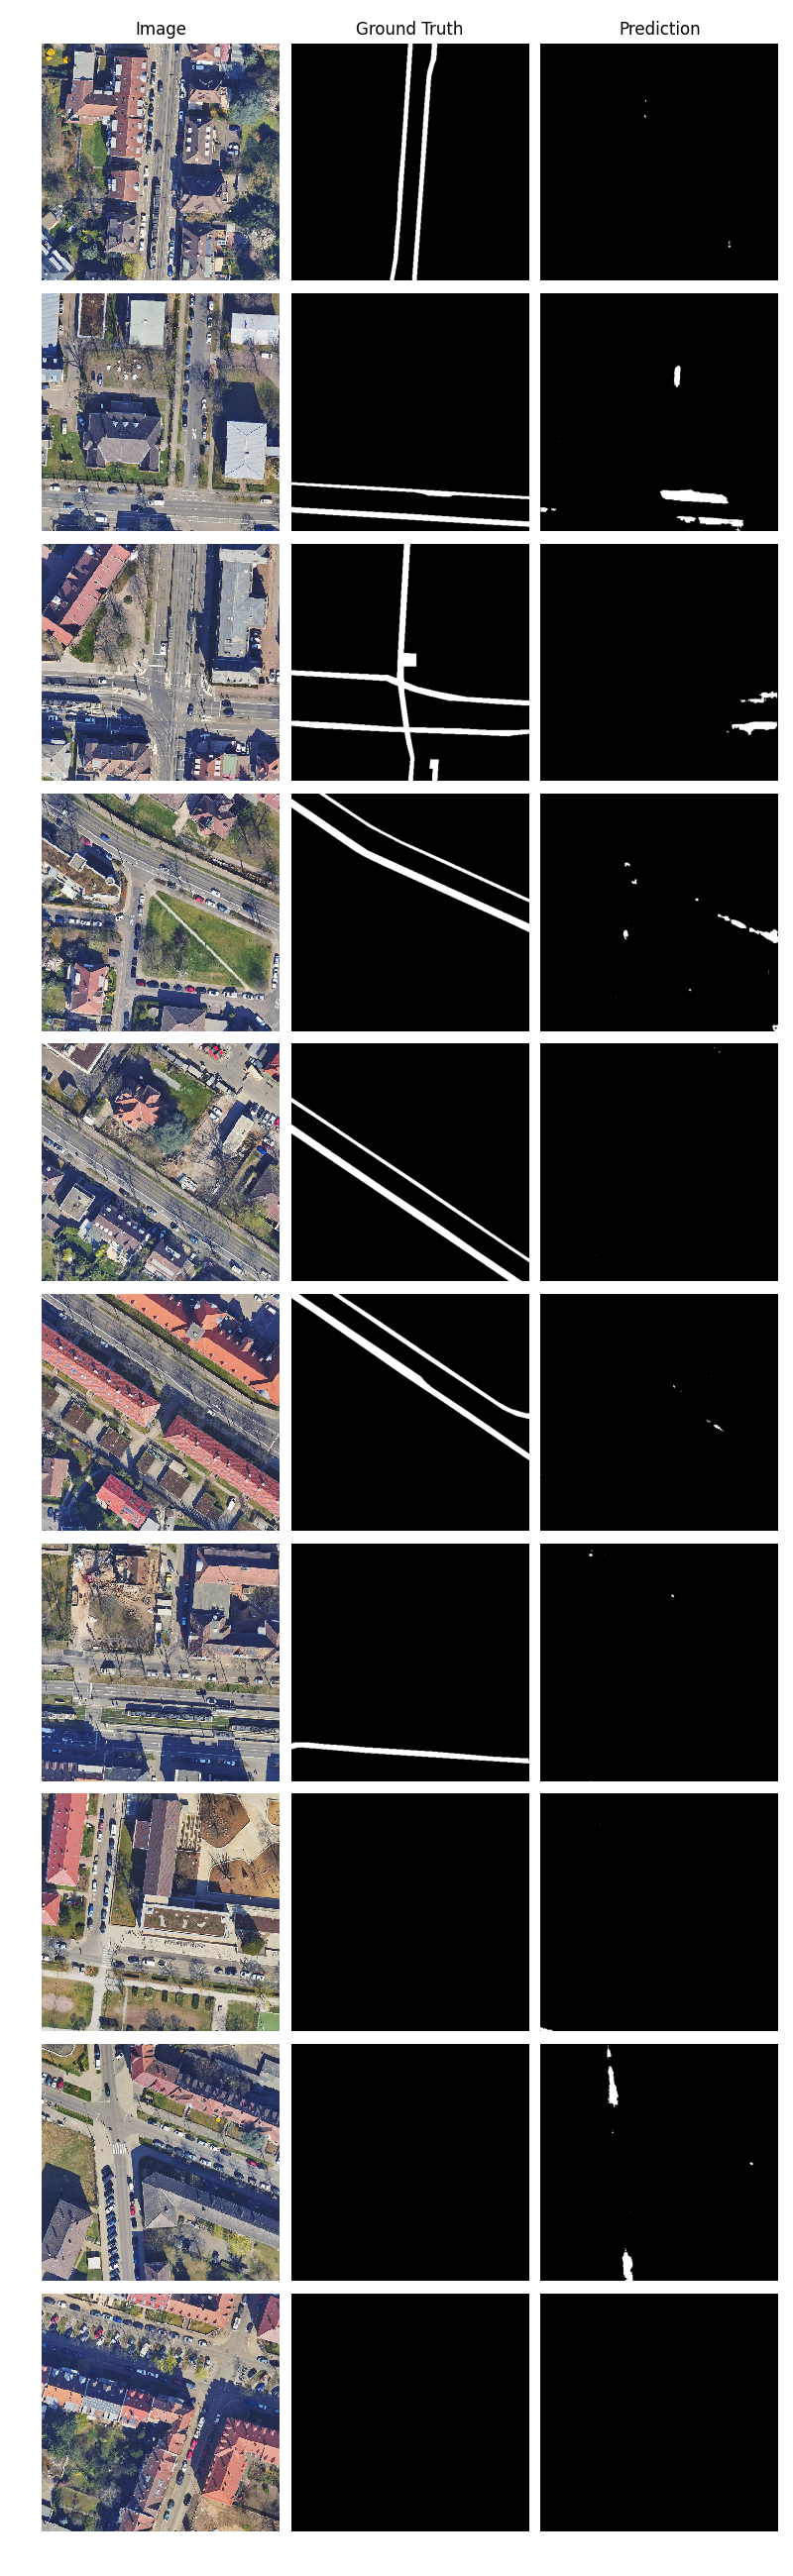
\includegraphics[width=.41\textwidth]{Bilder/Samples-KA/bunet2-l.png} 
	\caption{Beispiel-Predictions des $BUNet2^l$ auf dem Karlsruhe-Datensatz.}
	\label{fig:ka-samples-bunet2-l}
\end{figure}

\begin{figure}
	\centering
	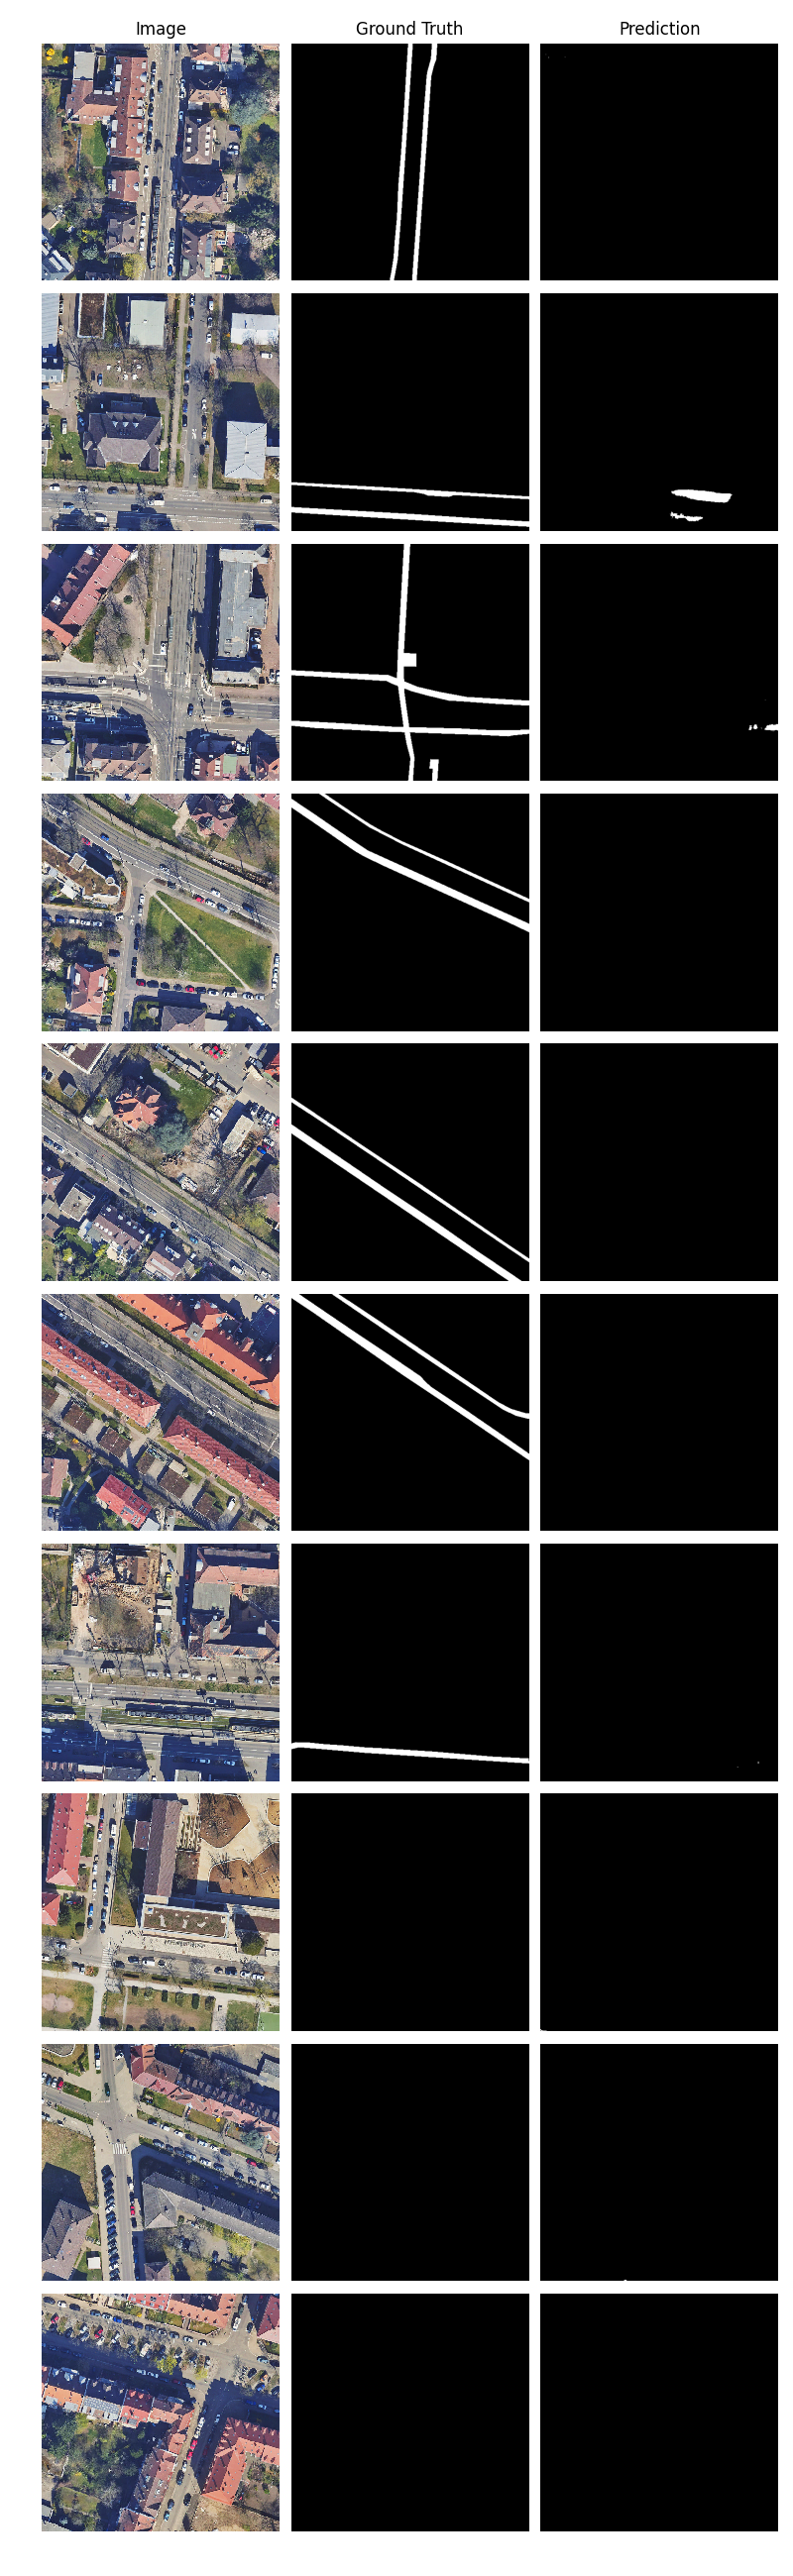
\includegraphics[width=.41\textwidth]{Bilder/Samples-KA/bunet2-r.png} 
	\caption{Beispiel-Predictions des $BUNet2^r$ auf dem Karlsruhe-Datensatz.}
	\label{fig:ka-samples-bunet2-r}
\end{figure}

\begin{figure}
	\centering
	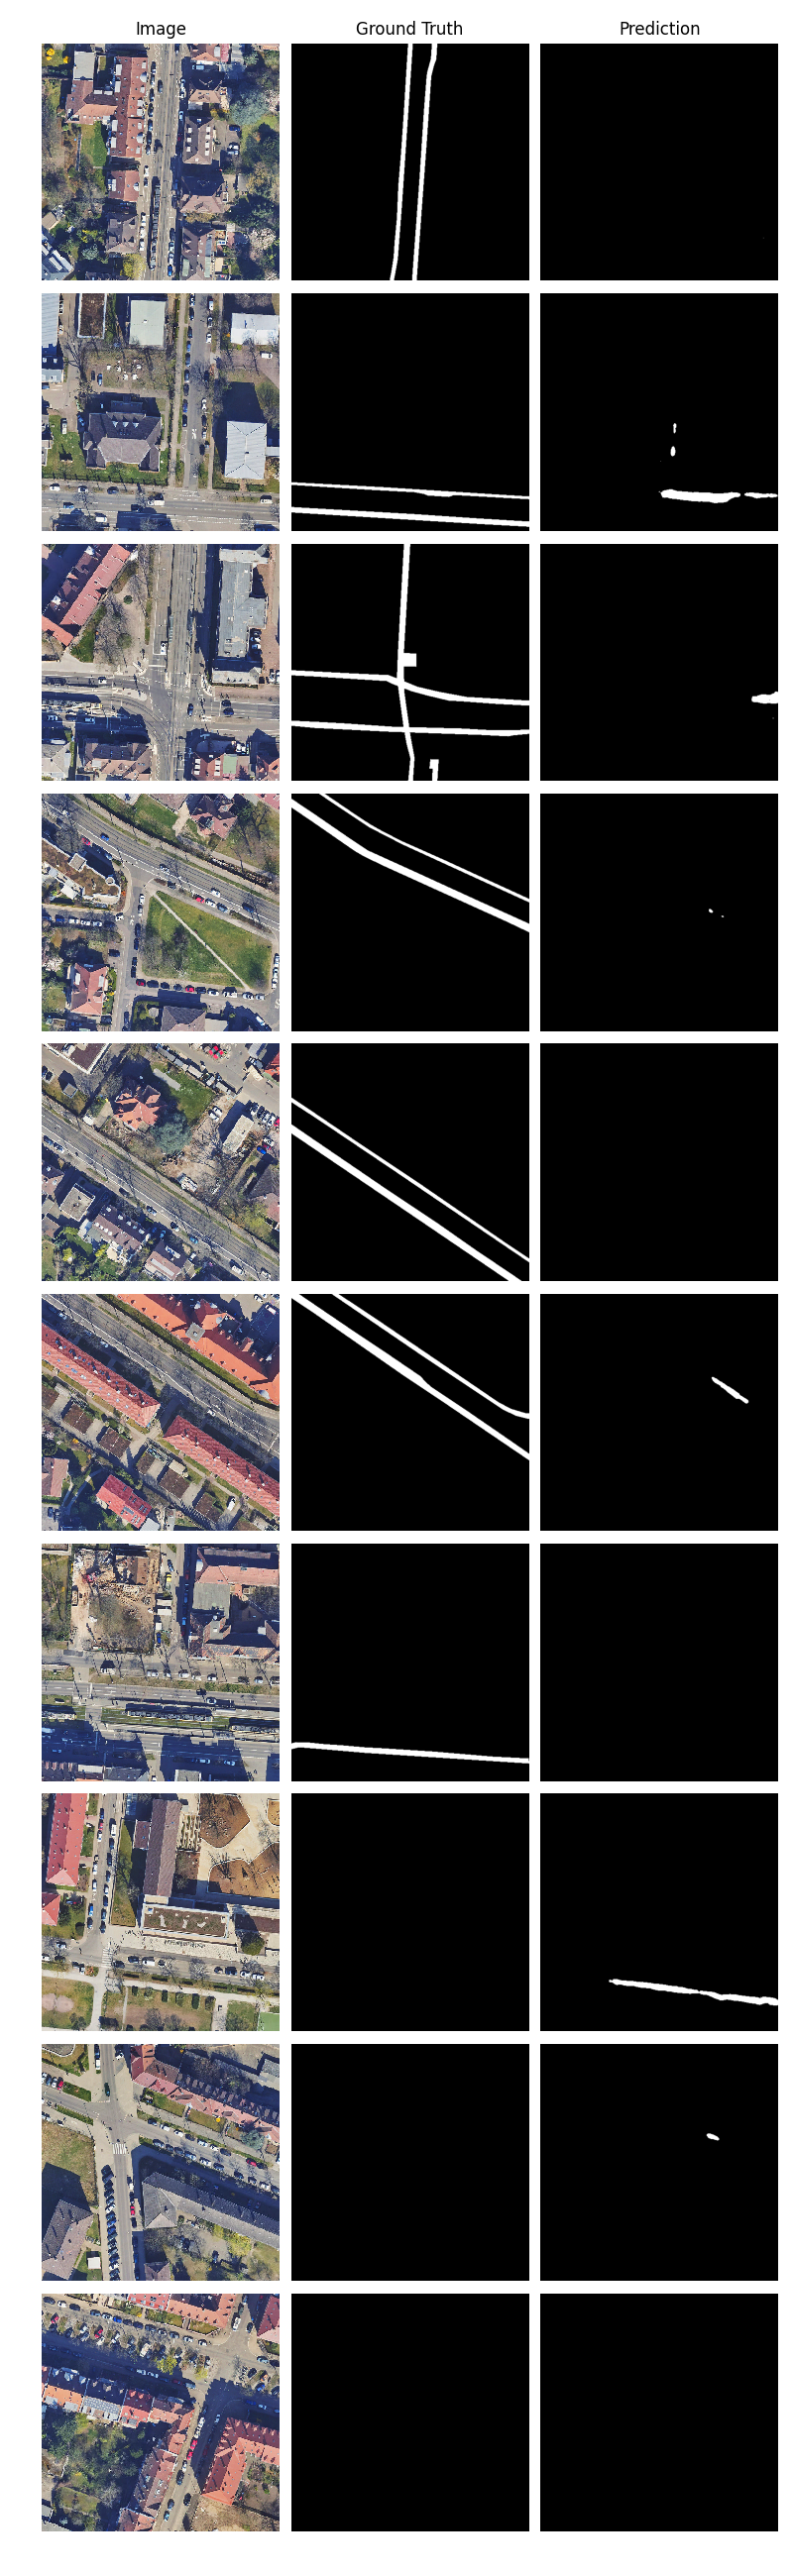
\includegraphics[width=.41\textwidth]{Bilder/Samples-KA/bunet2-s.png} 
	\caption{Beispiel-Predictions des $BUNet2^*$ auf dem Karlsruhe-Datensatz.}
	\label{fig:ka-samples-bunet2-s}
\end{figure}

\begin{figure}
	\centering
	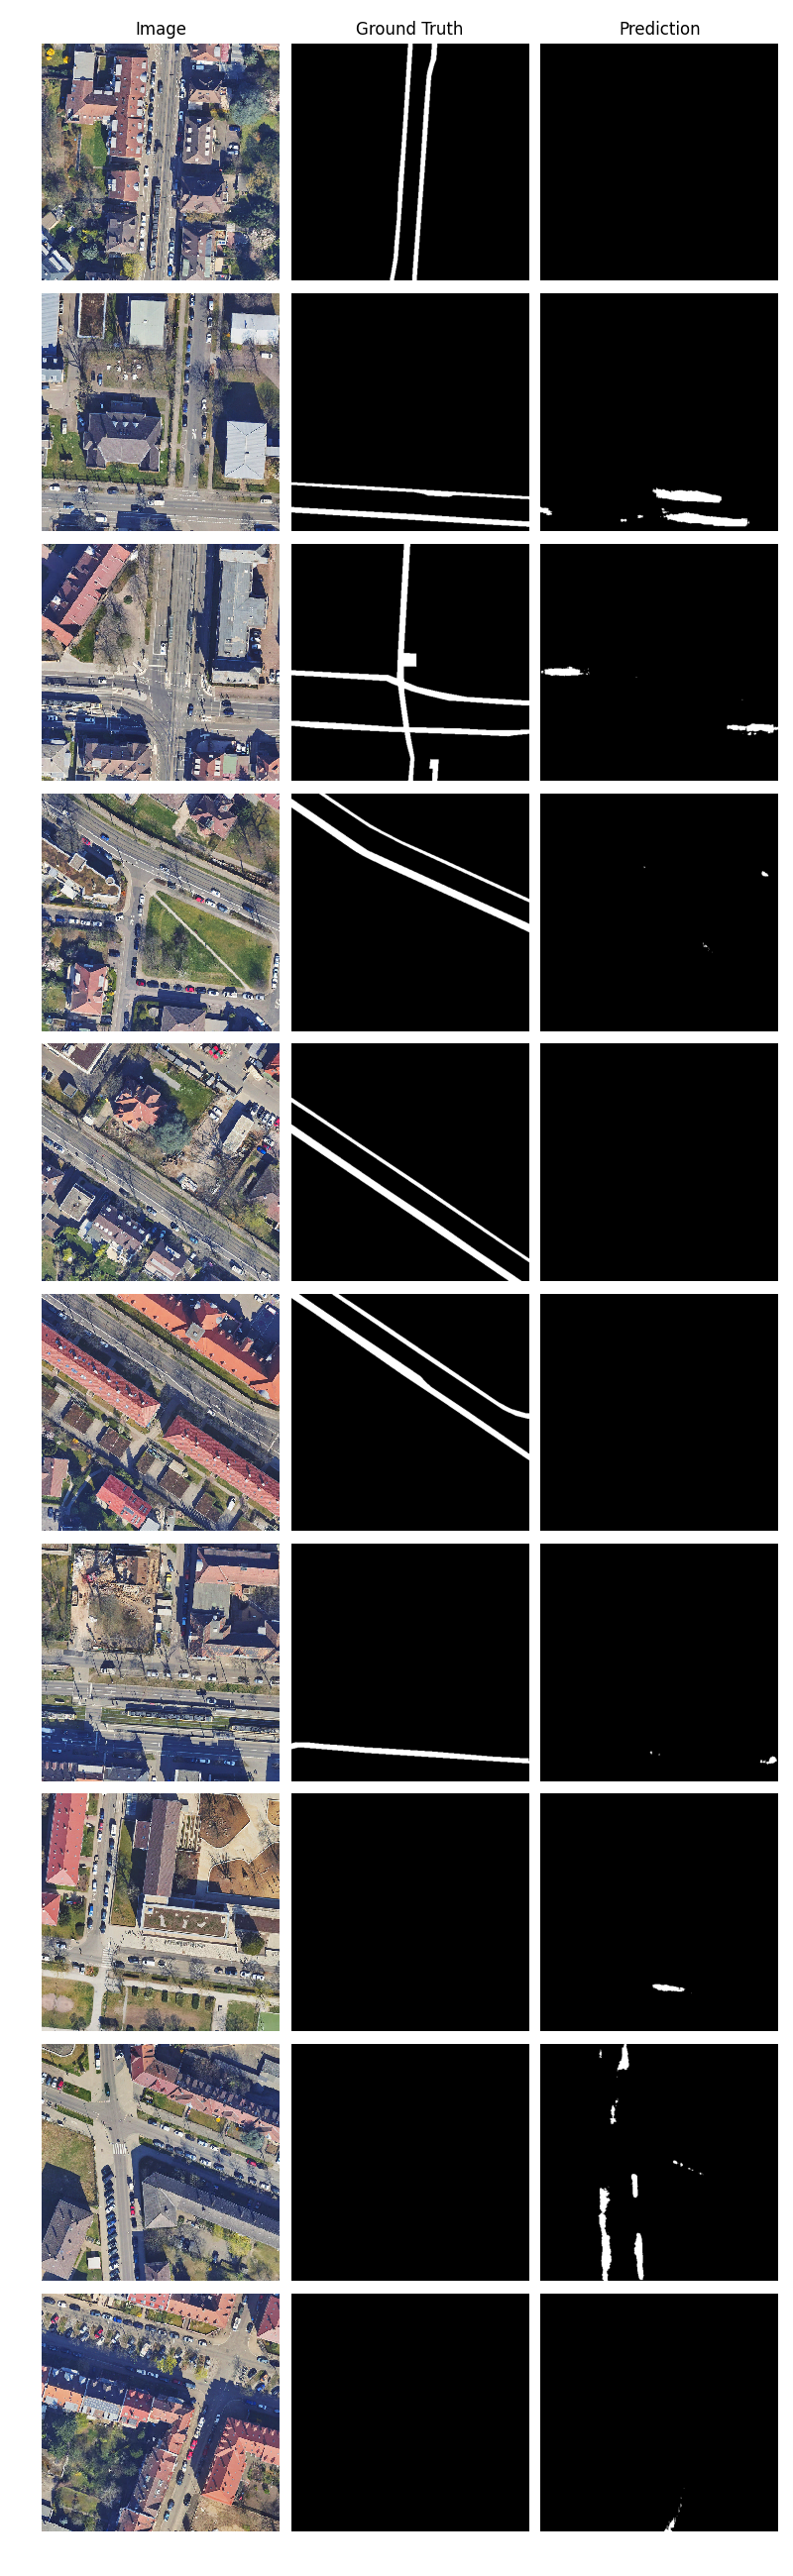
\includegraphics[width=.41\textwidth]{Bilder/Samples-KA/bunet15-l.png} 
	\caption{Beispiel-Predictions des $BUNet15^l$ auf dem Karlsruhe-Datensatz.}
	\label{fig:ka-samples-bunet15-l}
\end{figure}

\begin{figure}
	\centering
	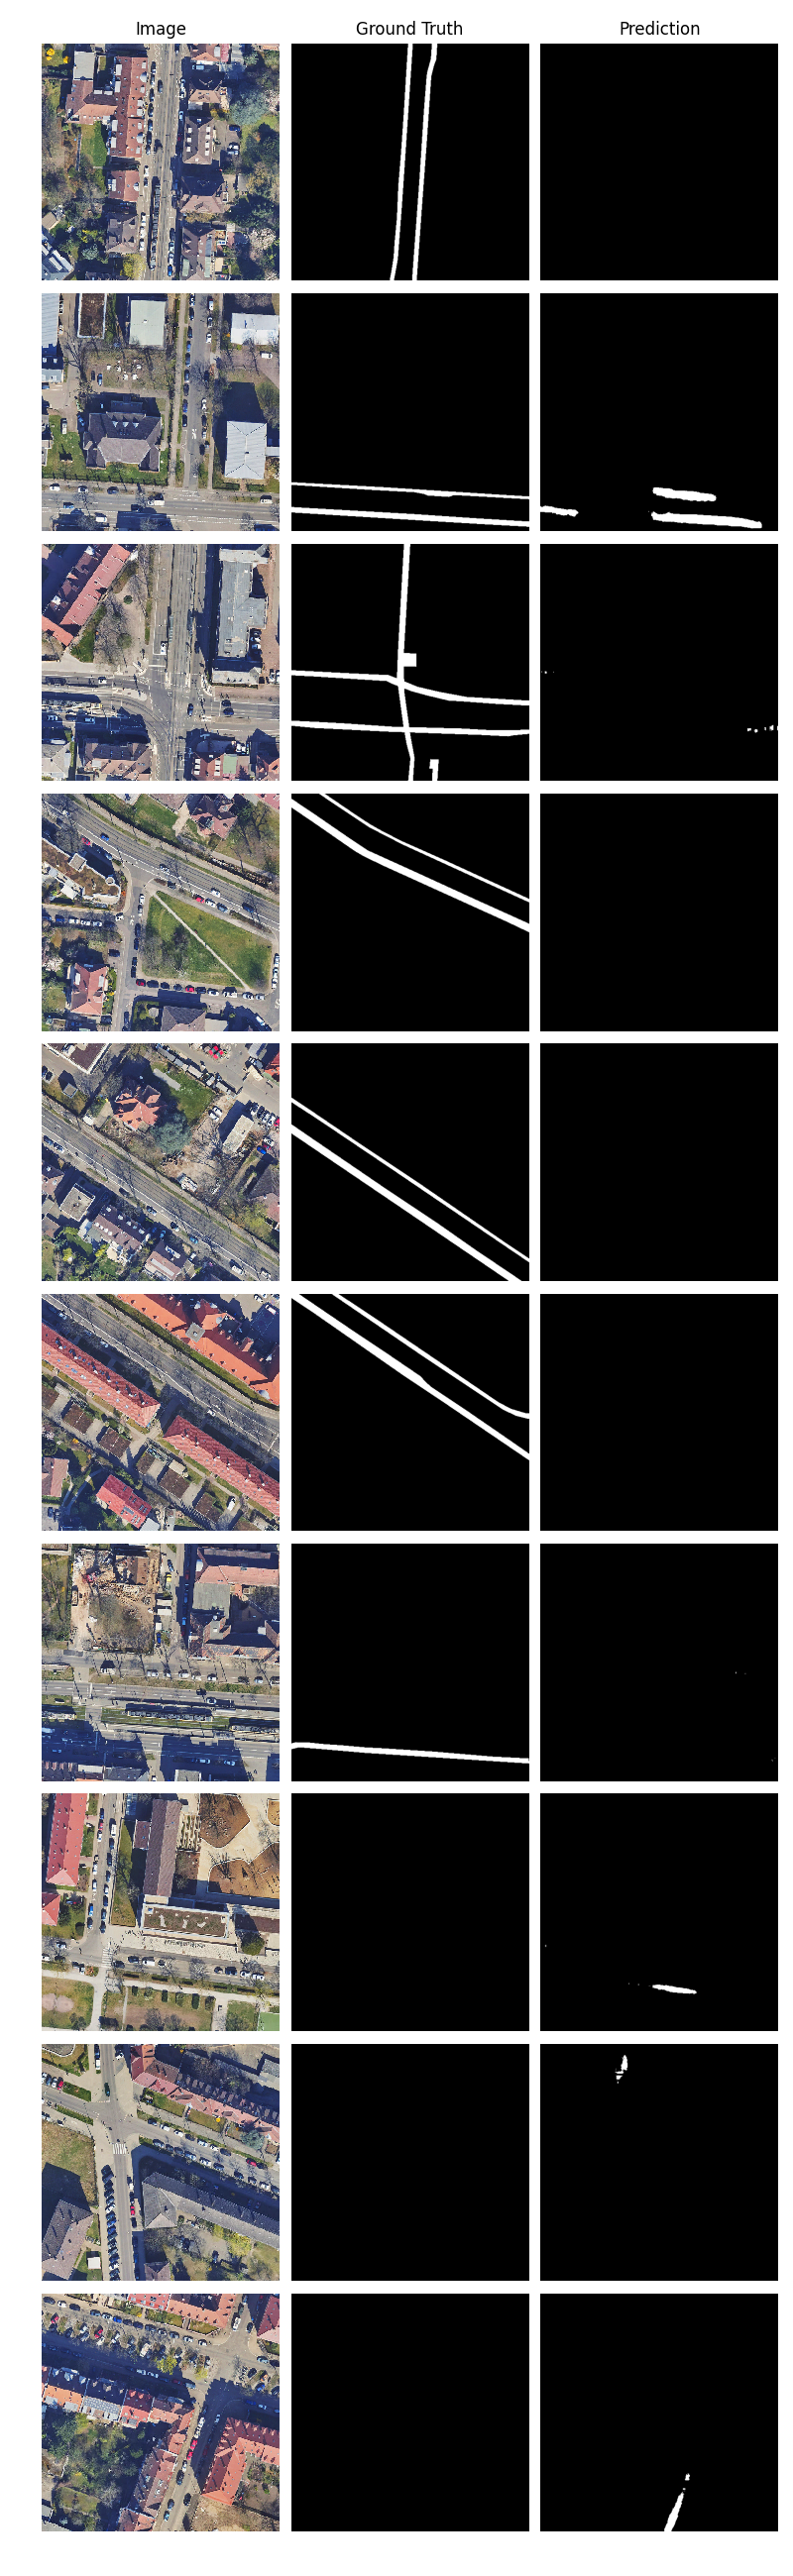
\includegraphics[width=.41\textwidth]{Bilder/Samples-KA/bunet15-r.png} 
	\caption{Beispiel-Predictions des $BUNet15^r$ auf dem Karlsruhe-Datensatz.}
	\label{fig:ka-samples-bunet15-r}
\end{figure}

\begin{figure}
	\centering
	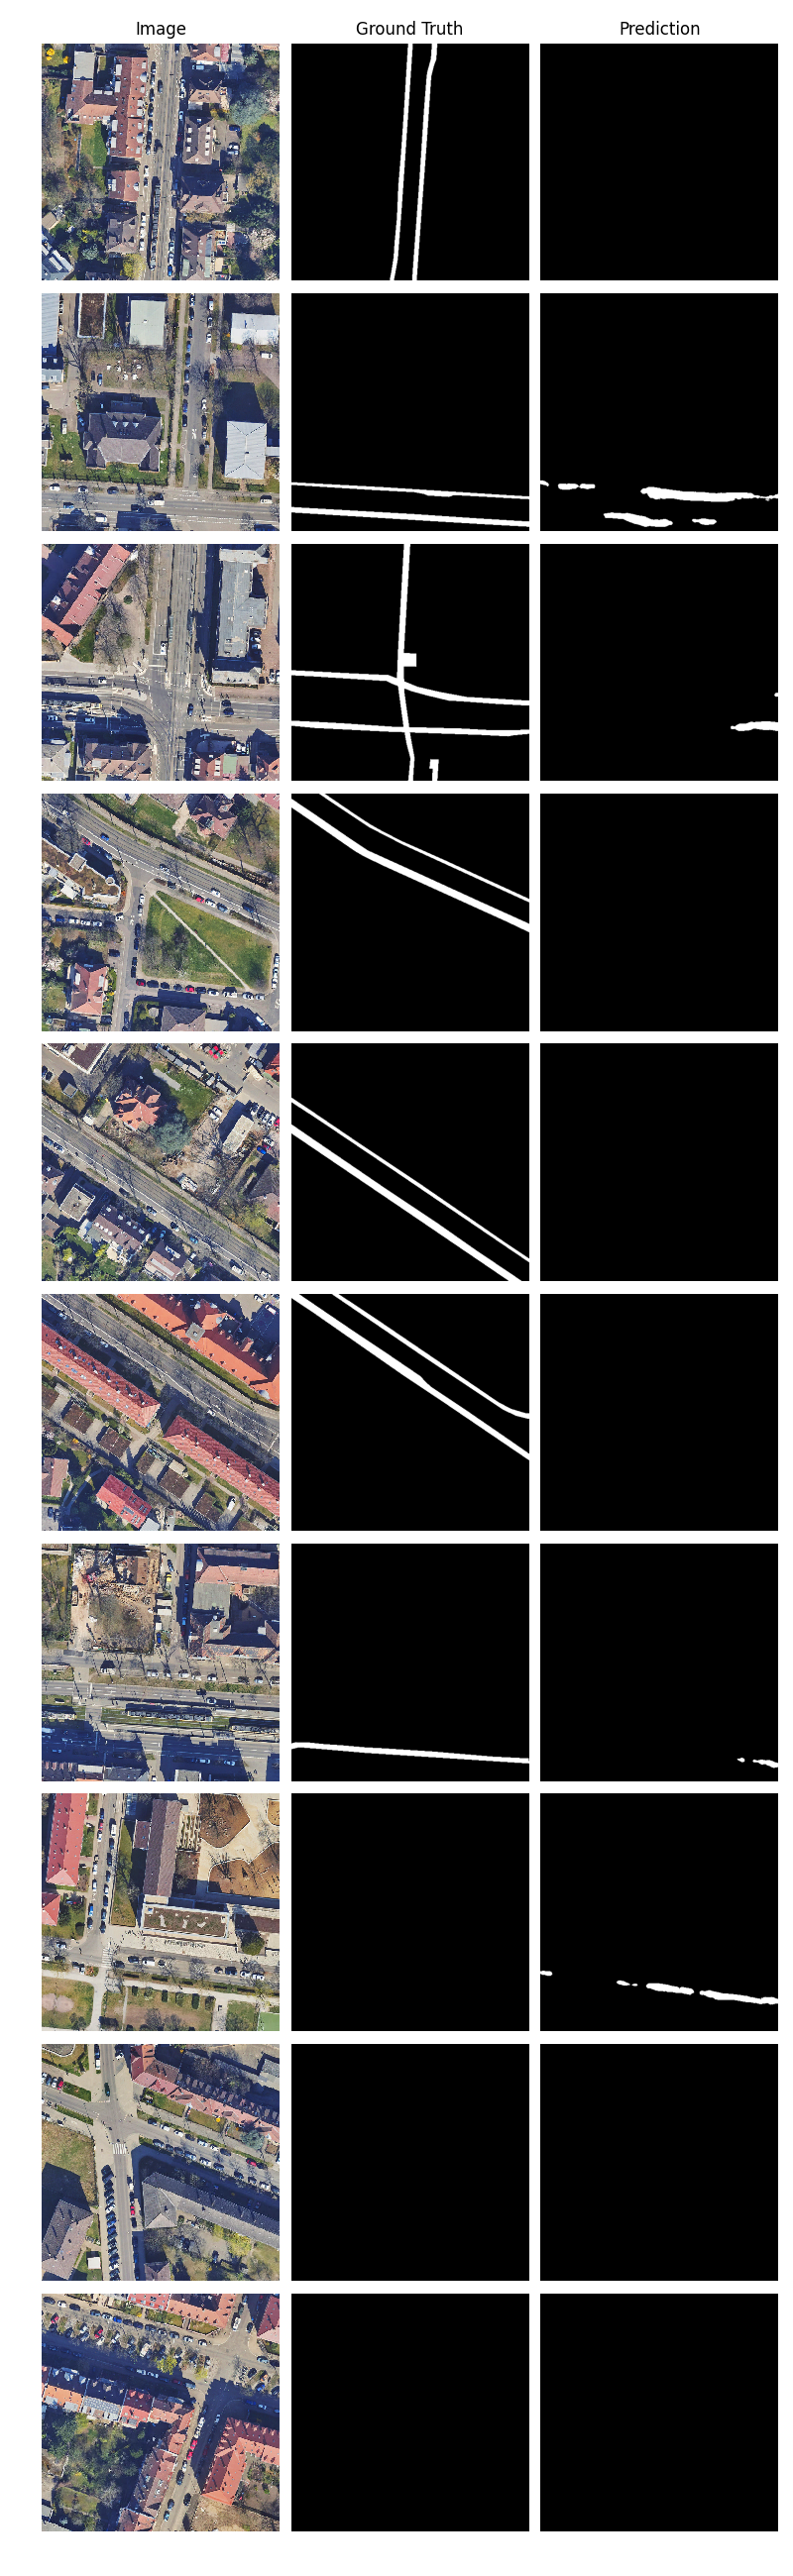
\includegraphics[width=.41\textwidth]{Bilder/Samples-KA/bunet15-s.png} 
	\caption{Beispiel-Predictions des $BUNet15^*$ auf dem Karlsruhe-Datensatz.}
	\label{fig:ka-samples-bunet15-s}
\end{figure}

\begin{figure}
	\centering
	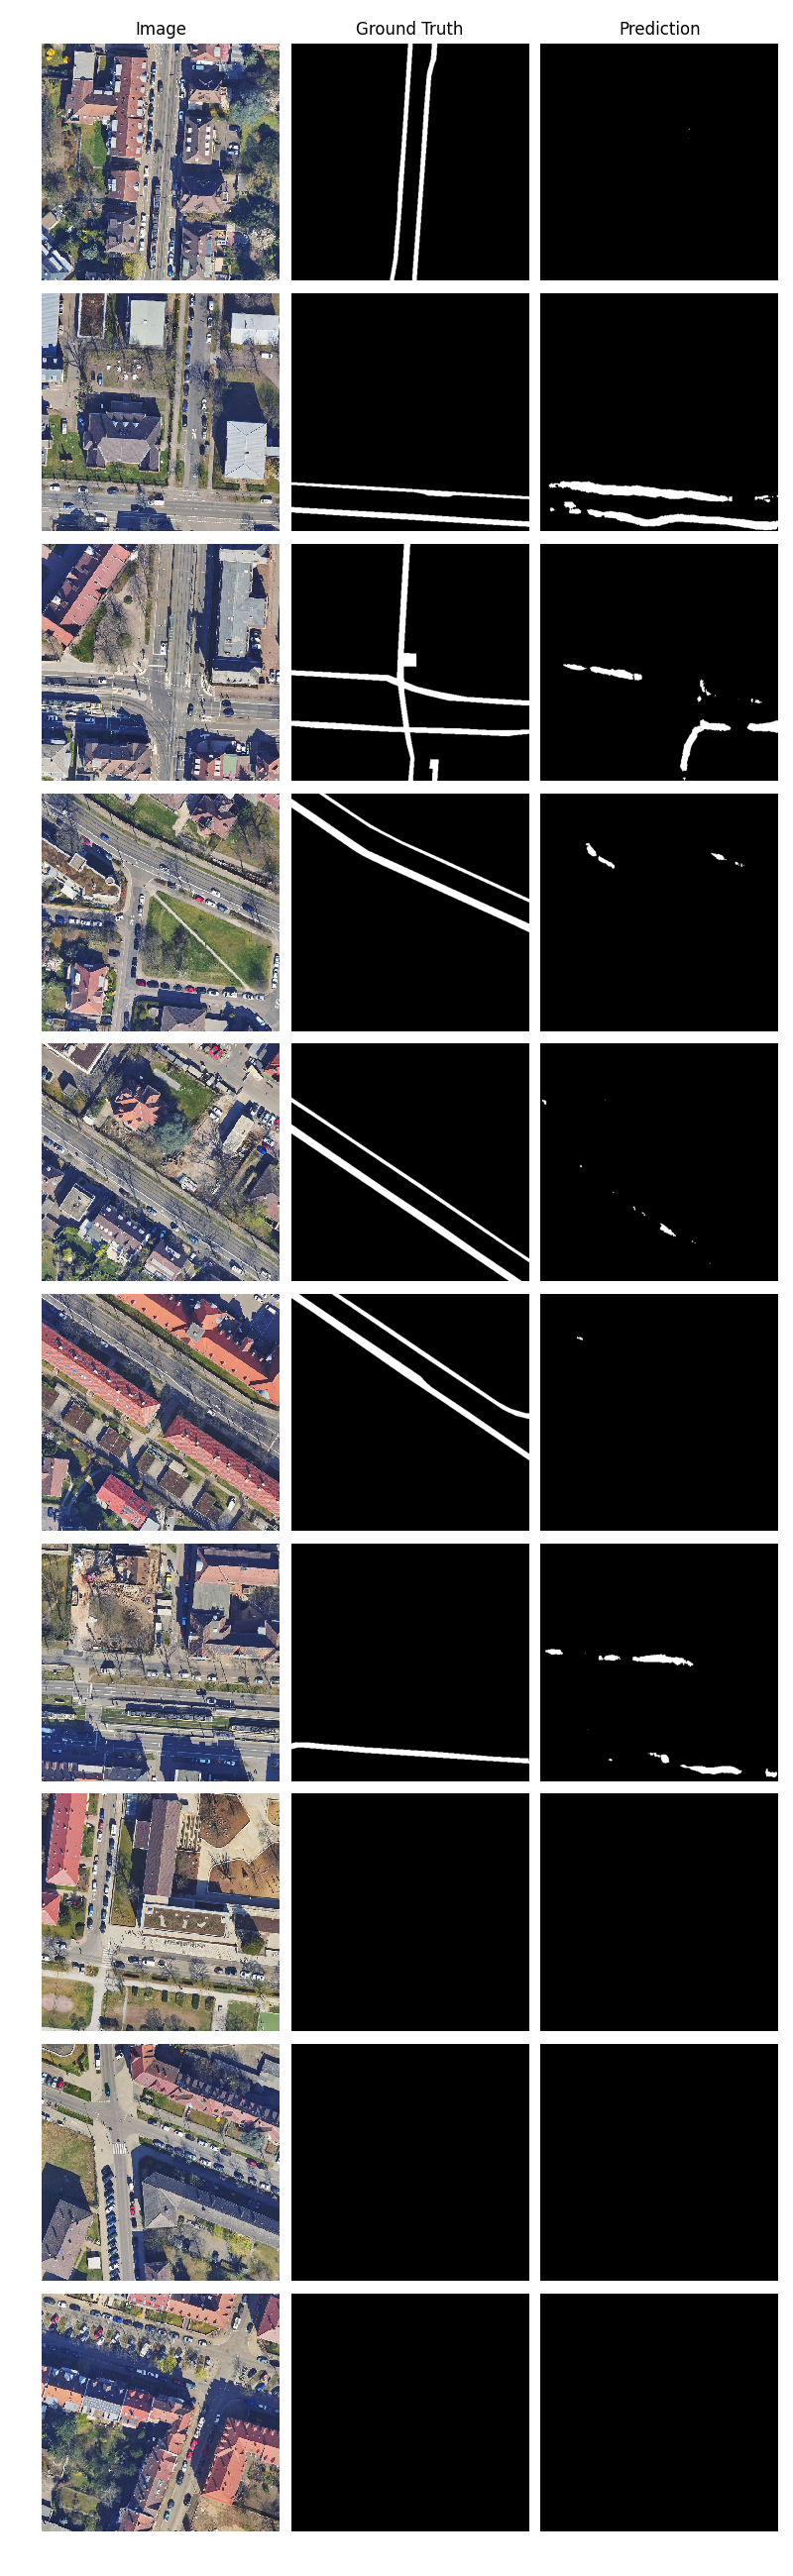
\includegraphics[width=.41\textwidth]{Bilder/Samples-KA/dbunet-l.png} 
	\caption{Beispiel-Predictions des $DBUNet^l$ auf dem Karlsruhe-Datensatz.}
	\label{fig:ka-samples-dbunet-l}
\end{figure}

\begin{figure}
	\centering
	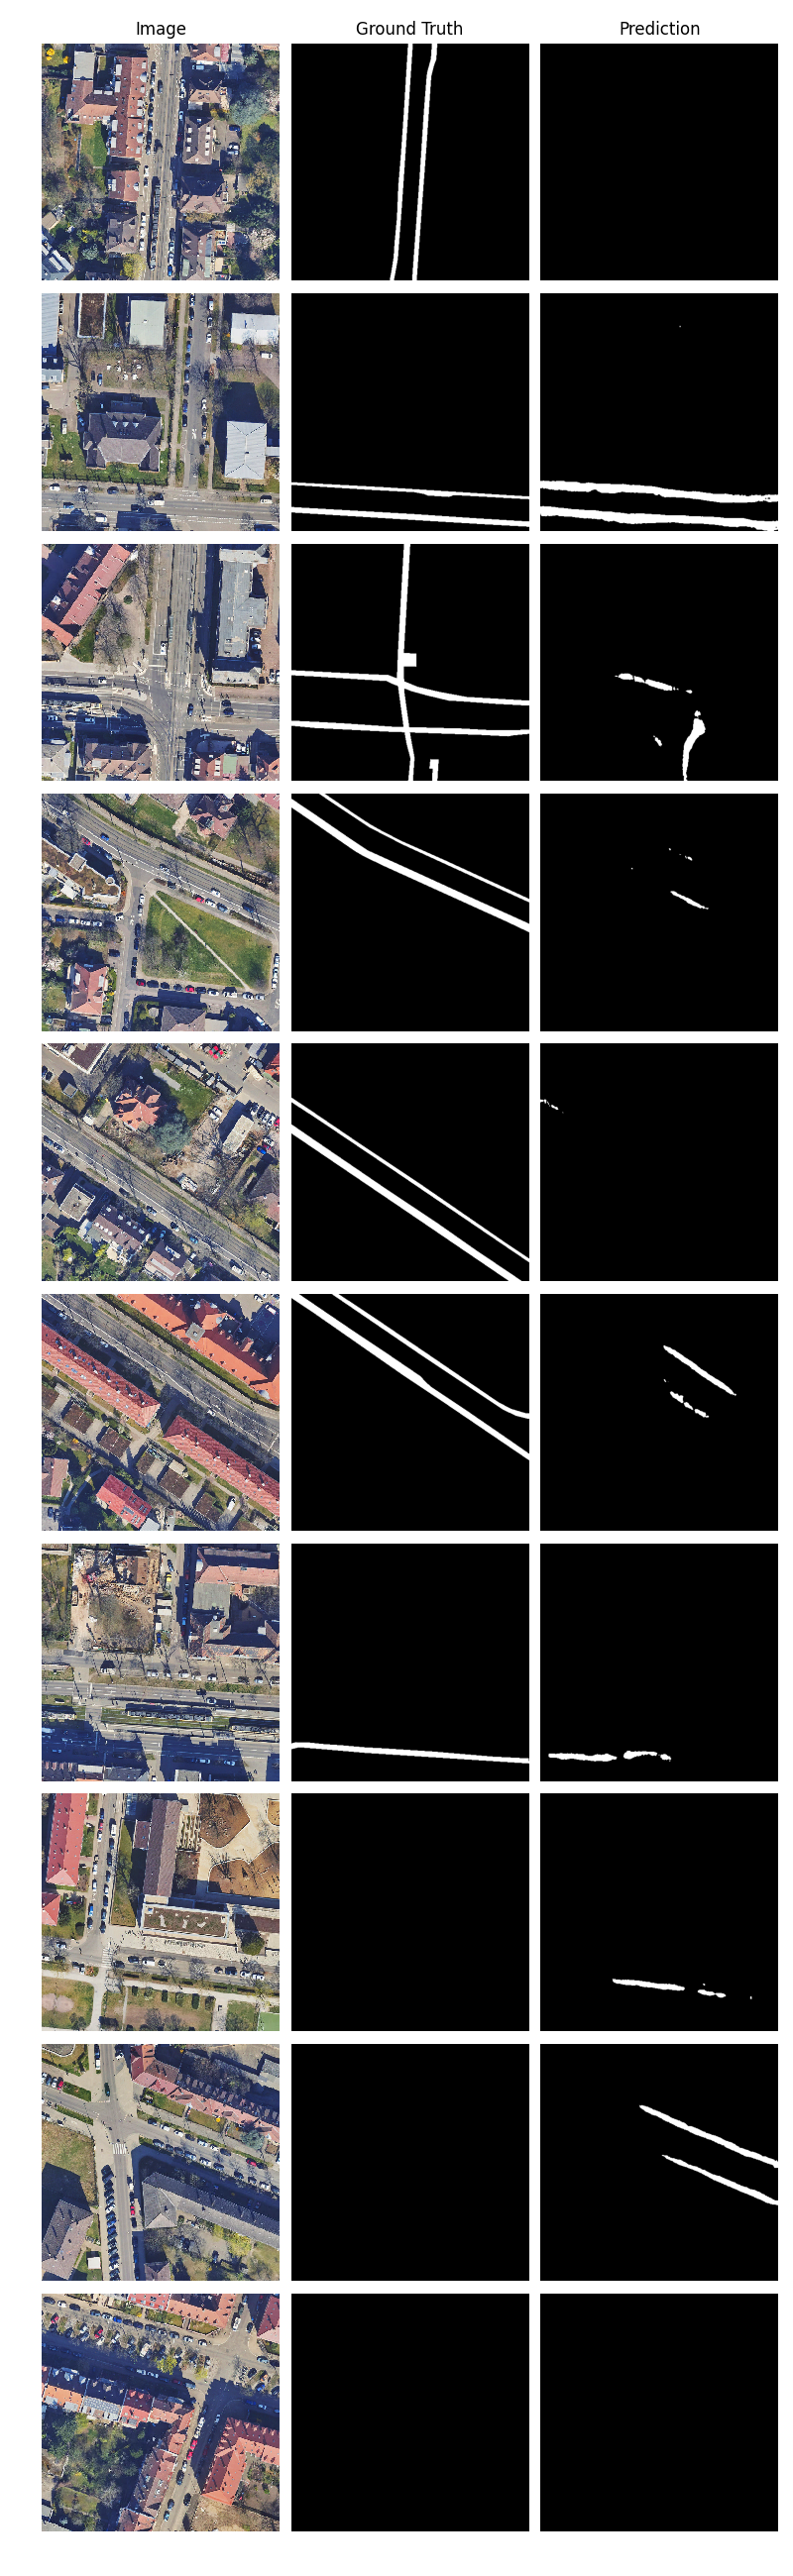
\includegraphics[width=.41\textwidth]{Bilder/Samples-KA/dbunet-r.png} 
	\caption{Beispiel-Predictions des $DBUNet^r$ auf dem Karlsruhe-Datensatz.}
	\label{fig:ka-samples-dbunet-r}
\end{figure}

\begin{figure}
	\centering
	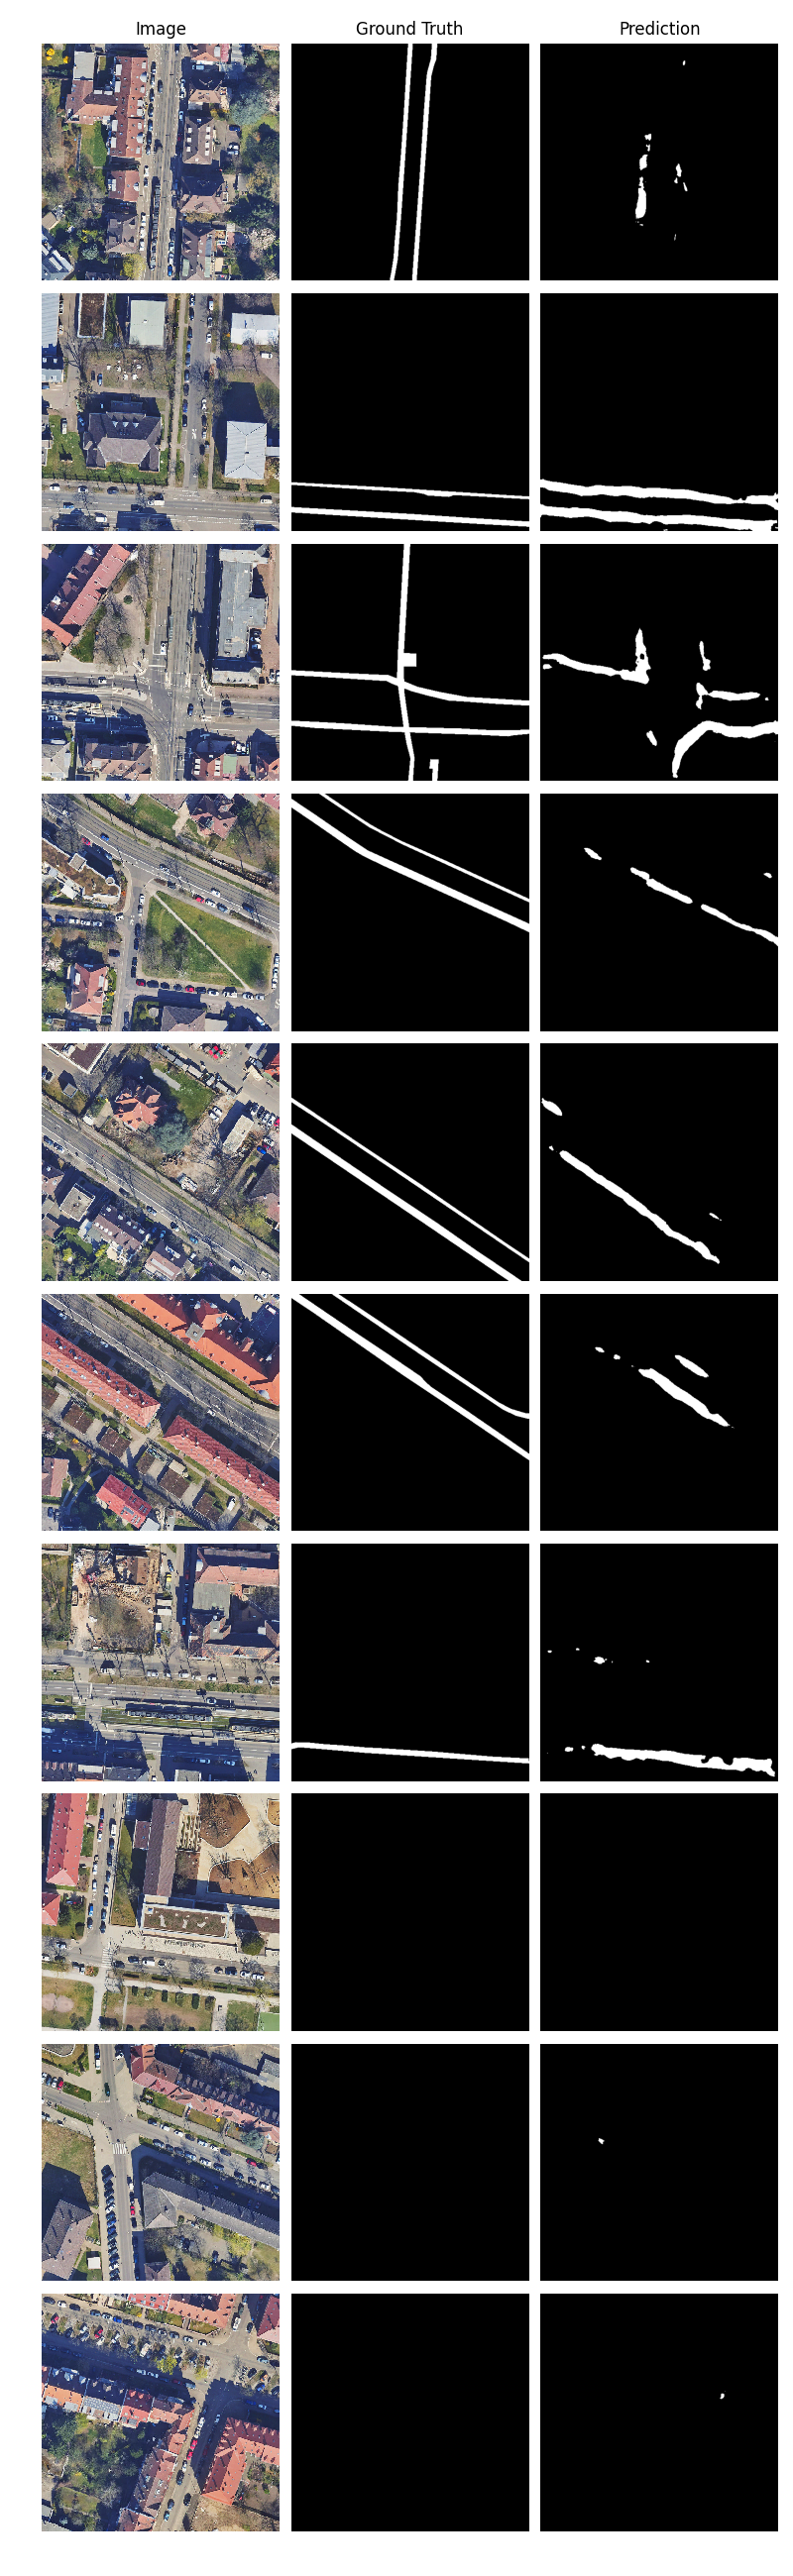
\includegraphics[width=.41\textwidth]{Bilder/Samples-KA/dbunet-s.png} 
	\caption{Beispiel-Predictions des $DBUNet^*$ auf dem Karlsruhe-Datensatz.}
	\label{fig:ka-samples-dbunet-s}
\end{figure}



\begin{figure}
	\centering
	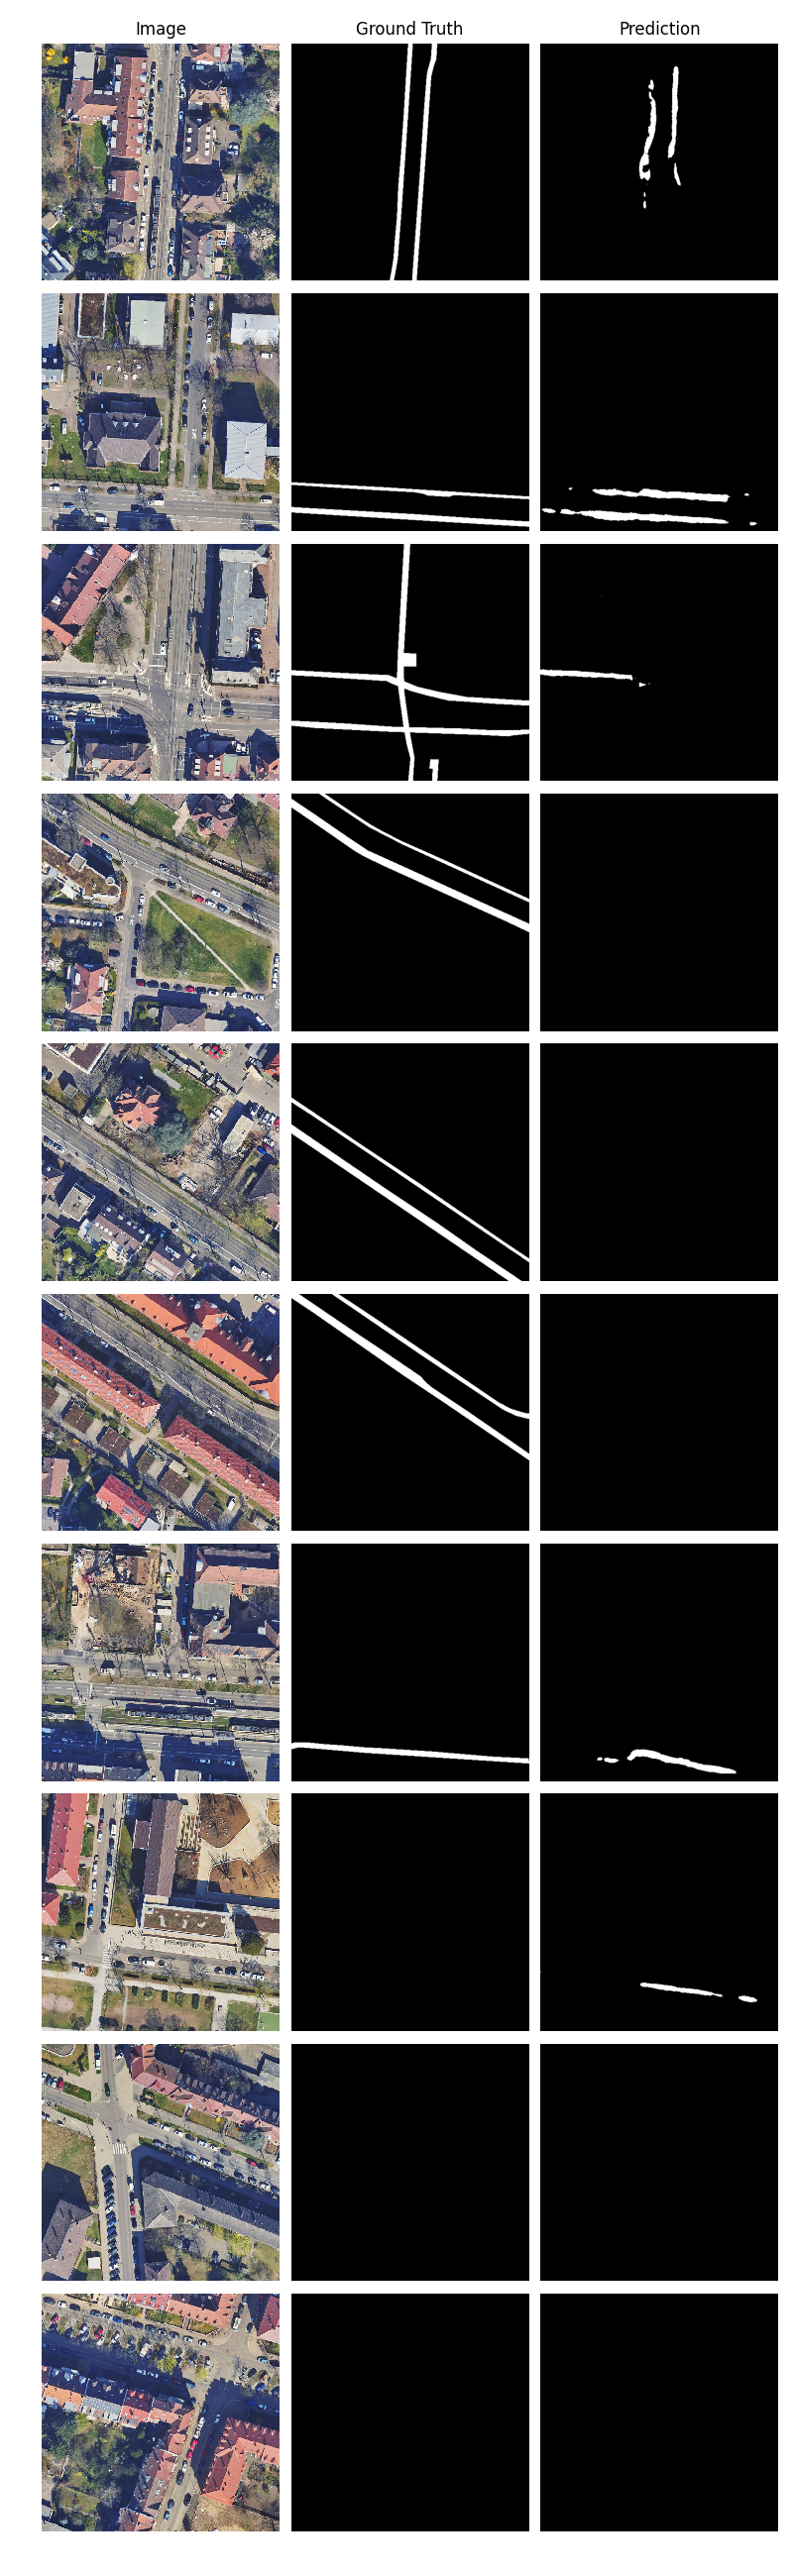
\includegraphics[width=.41\textwidth]{Bilder/Samples-KA/rbunet-r.png} 
	\caption{Beispiel-Predictions des $RBUNet^r$ auf dem Karlsruhe-Datensatz.}
	\label{fig:ka-samples-rbunet-r}
\end{figure}

\begin{figure}
	\centering
	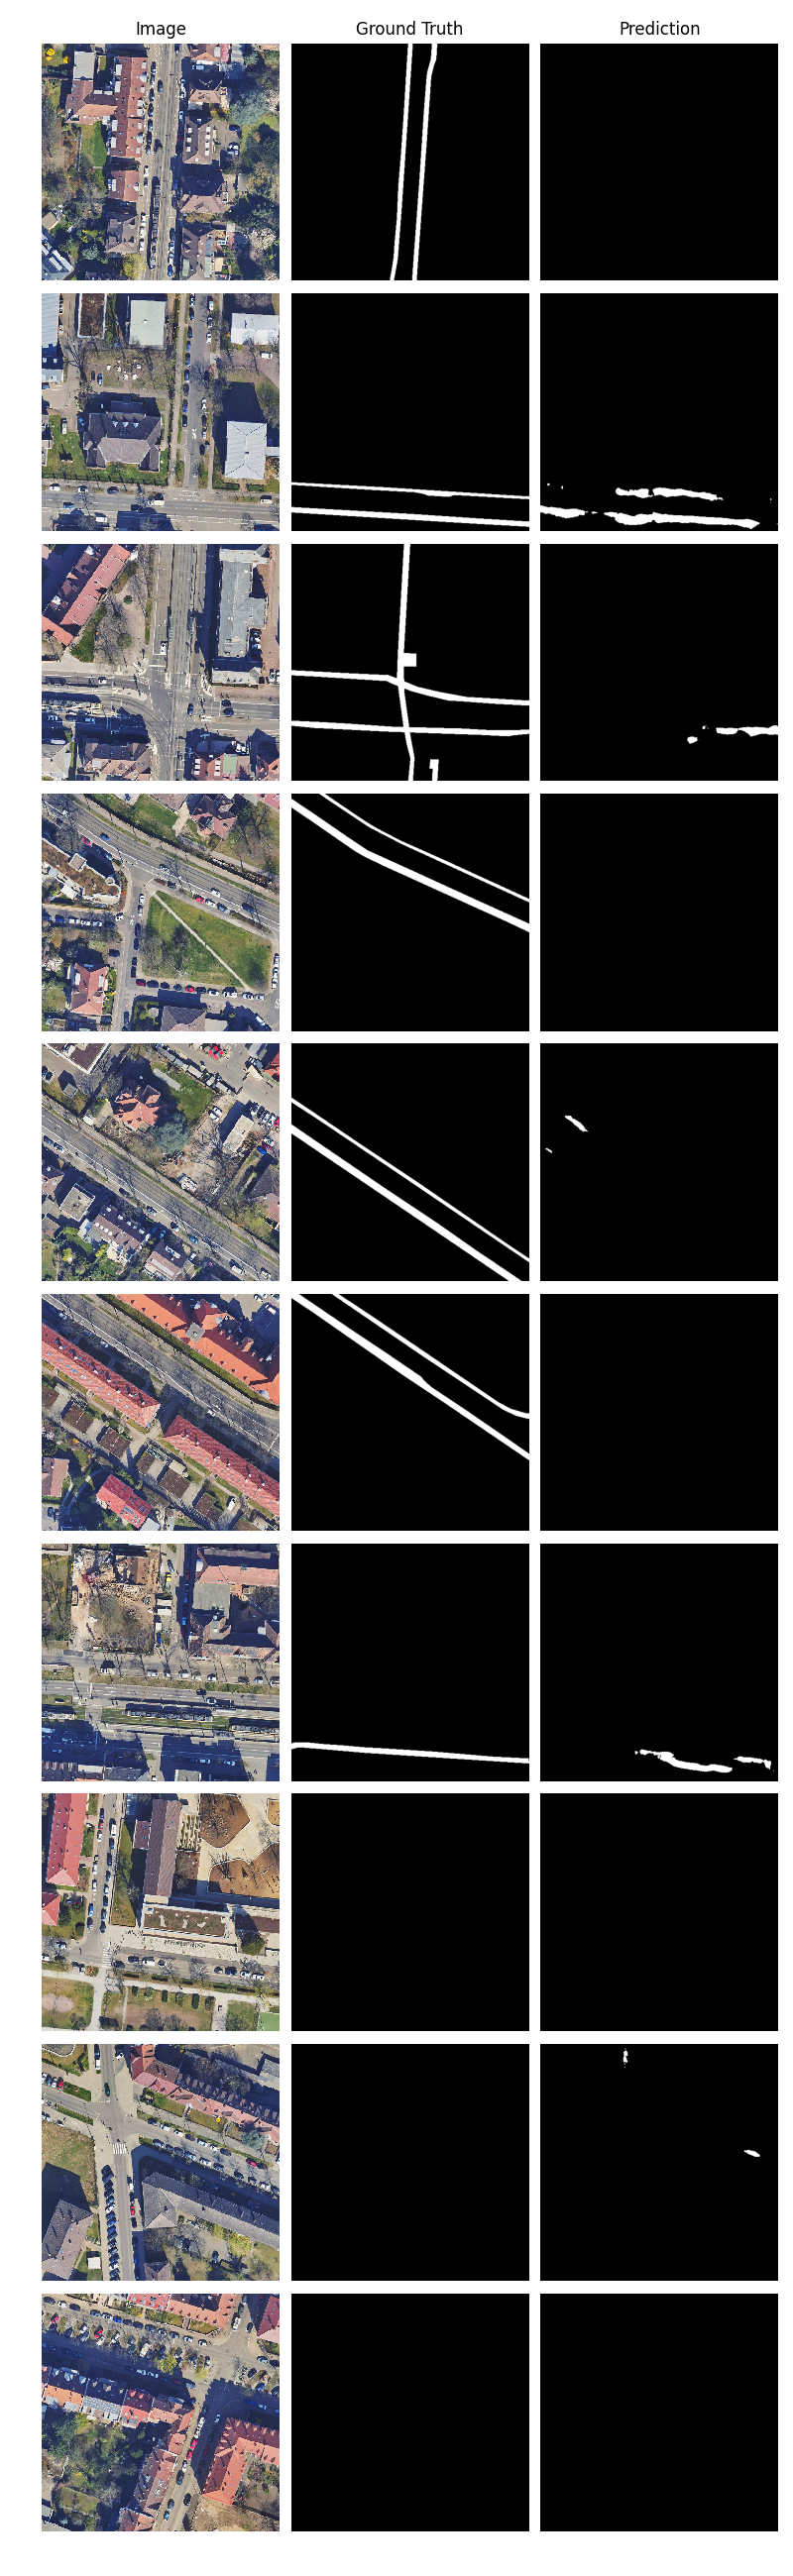
\includegraphics[width=.41\textwidth]{Bilder/Samples-KA/vbunet-l.png} 
	\caption{Beispiel-Predictions des $VBUNet^l$ auf dem Karlsruhe-Datensatz.}
	\label{fig:ka-samples-vbunet-l}
\end{figure}

\begin{figure}
	\centering
	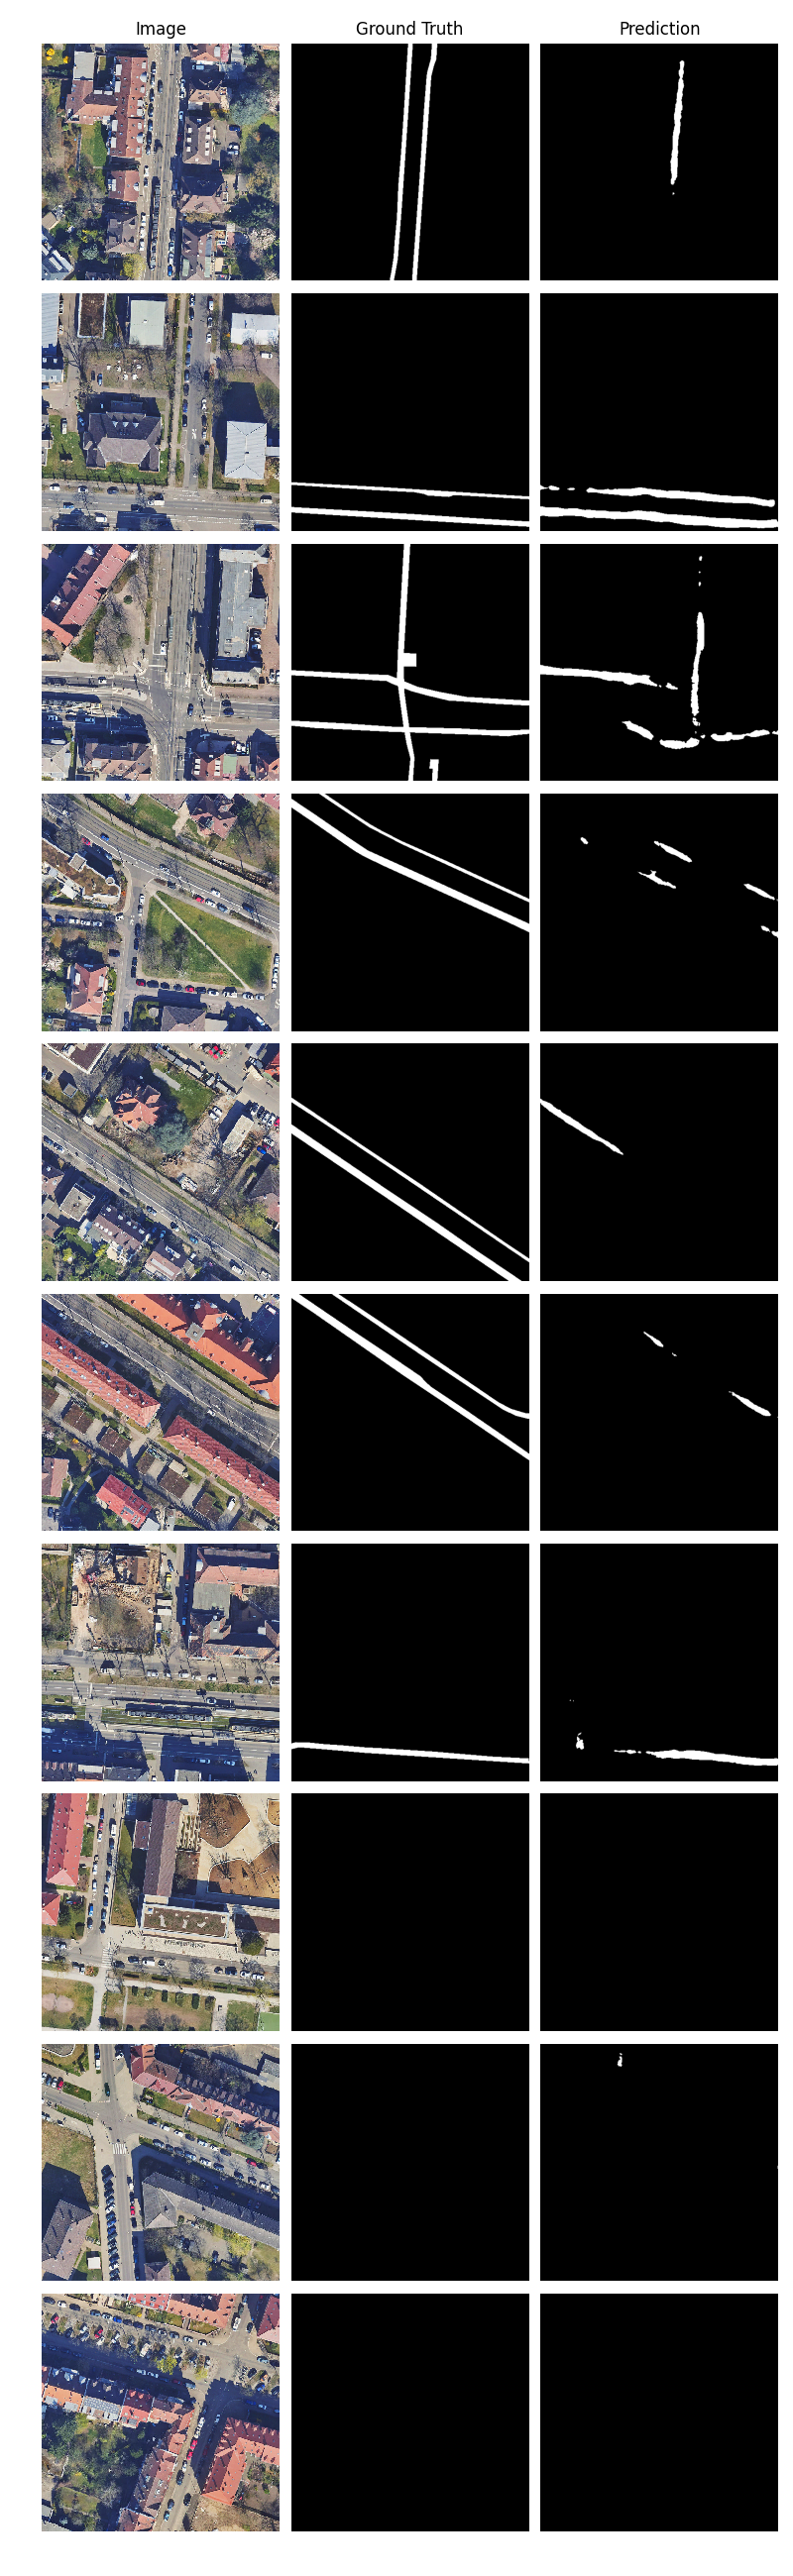
\includegraphics[width=.41\textwidth]{Bilder/Samples-KA/vbunet-r.png} 
	\caption{Beispiel-Predictions des $VBUNet^r$ auf dem Karlsruhe-Datensatz.}
	\label{fig:ka-samples-vbunet-r}
\end{figure}

\begin{figure}
	\centering
	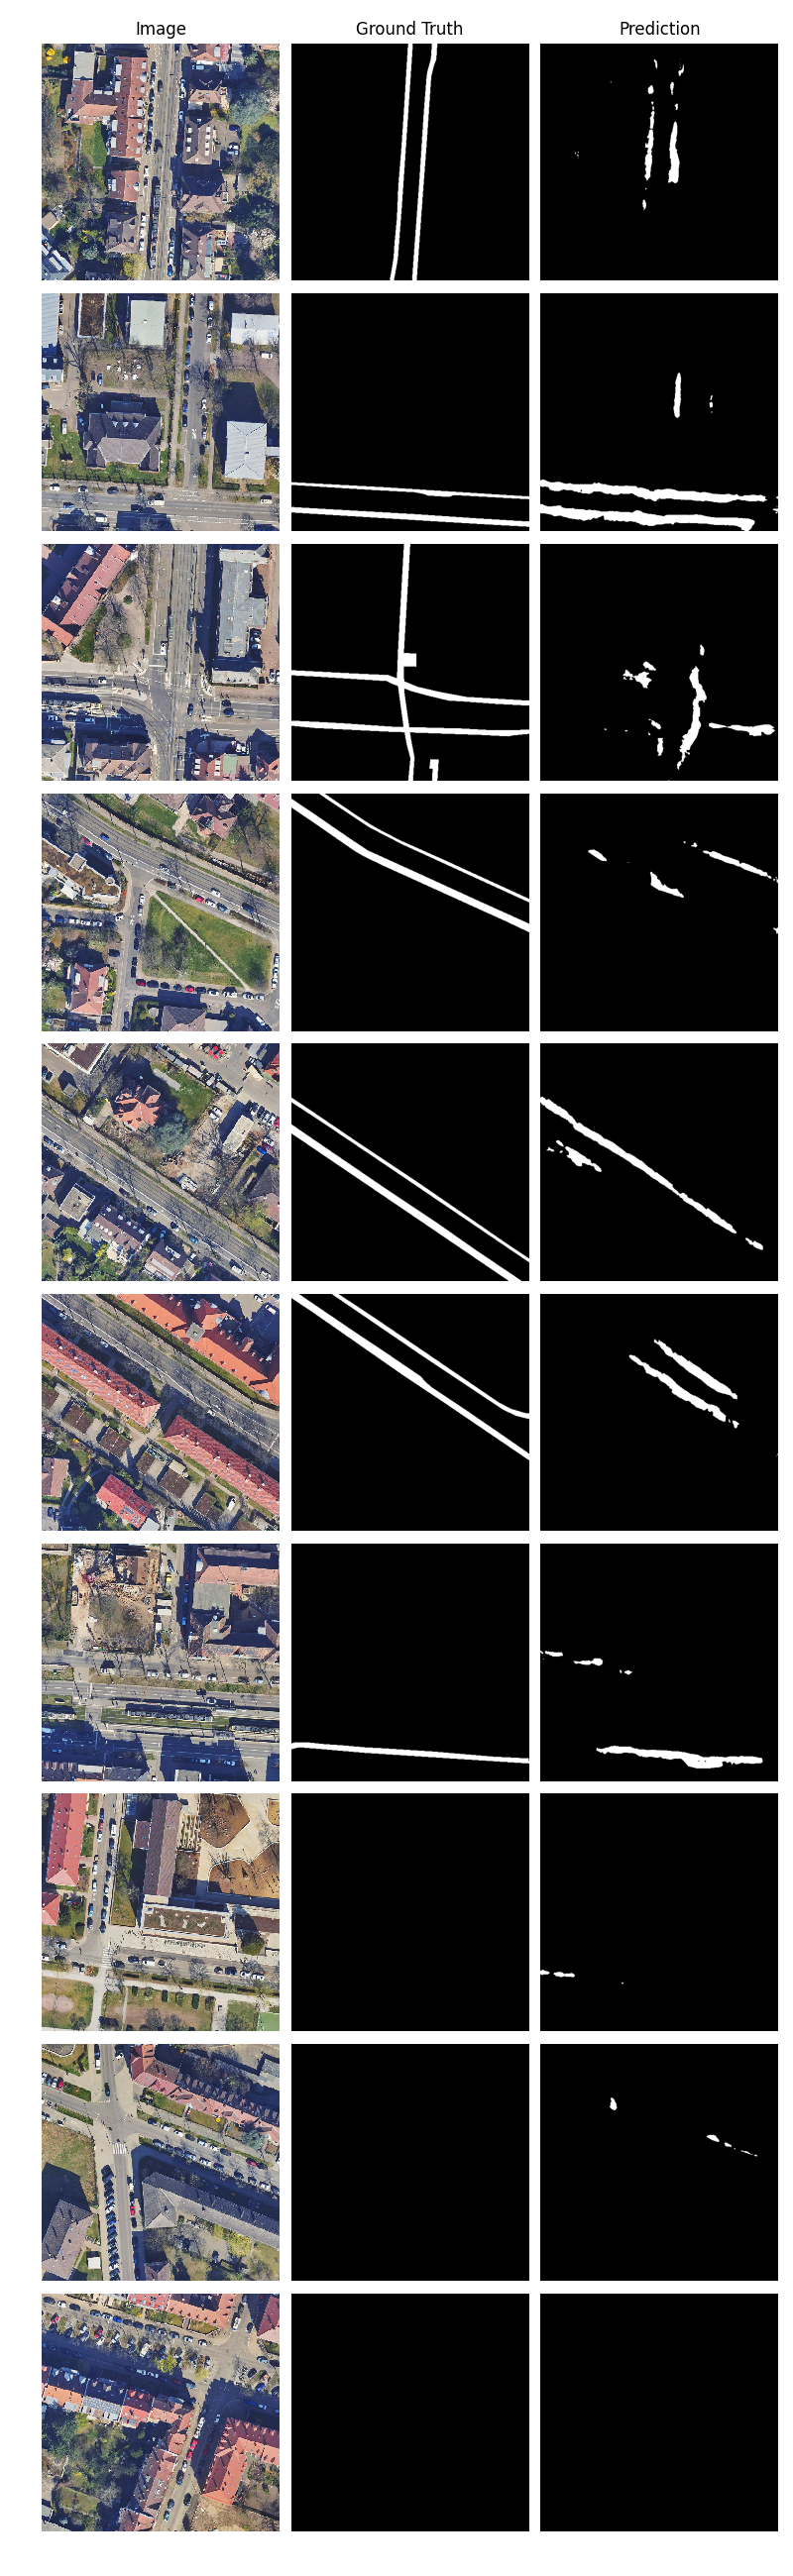
\includegraphics[width=.41\textwidth]{Bilder/Samples-KA/vbunet-s.png} 
	\caption{Beispiel-Predictions des $VBUNet^*$ auf dem Karlsruhe-Datensatz.}
	\label{fig:ka-samples-vbunet-s}
\end{figure}